\chapter{Logistic Regression}
\label{chap:logreg}
%=============================================================================

Everything so far has predicted a continuous number.  We now turn to
\emph{classification}, where the target is a label drawn from a finite set:
whether a tumour is malignant or benign, whether a credit card holder will
default, which of ten digits a handwritten image shows.  The change of target
forces a change of model and, more interestingly, a change of loss function --
and the new loss will turn out to follow from the same maximum-likelihood
argument that produced least squares in Section~\ref{sec:maxlikelihood}.

Logistic regression is the natural first classifier, and it occupies the same
position in this book that linear regression did.  It is simple enough that
everything can be computed, its cost function is convex so that the
optimisation theory of Chapter~\ref{chap:optim} applies without qualification,
and -- most importantly for what follows -- it is exactly a neural network with
no hidden layers.  The sigmoid we introduce here is an activation function,
the cross-entropy we derive here is the loss used to train classifiers
throughout deep learning, and the gradient we compute here reappears as the
last step of backpropagation.  A reader who understands this chapter
thoroughly has already met most of the ingredients of the next one.

%----------------------------------------------------------------------
\section{Classification problems}
\label{sec:classification}

\index{classification}
We consider the case where the responses $y_i$ are discrete and take values
from $k=0,\dots,K-1$, that is $K$ classes.  The goal is to predict the class
from the design matrix $\bm{X}\in\mathbb{R}^{n\times p}$ of
Eq.~(\ref{eq:1-designmatrix}), made of $n$ samples each carrying $p$ features,
and in particular to identify the classes of new, unseen samples.

We specialise for most of the chapter to two classes, with outputs $y_i=0$ and
$y_i=1$.  The outcome might represent whether a credit card holder defaults on
their debt,
\begin{equation}
  y_i = \begin{cases} 0 & \text{no},\\ 1 & \text{yes}. \end{cases}
  \label{eq:5-binarylabels}
\end{equation}

\paragraph{Why not simply use linear regression?}
Before introducing anything new, it is worth seeing why the machinery of
Chapter~\ref{chap:lreg} is not adequate.  We could fit the linear model
\begin{equation}
  \bm{y} = \bm{X}\bm{\theta} + \bm{\varepsilon}
  \label{eq:5-linearattempt}
\end{equation}
and classify by thresholding, predicting class $1$ when
$\tilde{y}_i>0.5$ and class $0$ otherwise.  Something like this can be made
to work, but it is unsatisfactory for a fundamental reason: the right-hand
side of Eq.~(\ref{eq:5-linearattempt}) takes values on the entire real axis,
while $y_i$ takes only the values $0$ and $1$.  A fitted value of $-3.7$ or
$+2.4$ has no interpretation.  Worse, a single distant point drags the fitted
line and moves the decision threshold, so that adding a strongly-classified
observation can cause a previously correct classification to flip.

One way to force a discrete output is to compose the linear model with a sign
function, $f(s_i)=1$ if $s_i\ge0$ and $0$ otherwise.  This is the
\emph{perceptron}, historically the first machine learning model and the
subject of the opening of the next chapter.  It is a \emph{hard} classifier:
each data point is assigned deterministically to a category.  In many
situations we would rather have a \emph{soft} classifier, one that outputs
the \emph{probability} of a given category.  Probabilities can be thresholded
when a decision is needed, but they also express confidence, they can be
combined with costs when different errors matter differently, and -- as we
shall see -- they lead to a differentiable cost function, which the step
function does not.

\paragraph{An illustration.}
Data on coronary heart disease (CHD) as a function of age make the point.
Plotting whether a person has had CHD ($y=1$) or not ($y=0$) against age gives
two horizontal bands of points, and a straight-line fit through them is
visibly meaningless.

\begin{Python}{}
import numpy as np
import pandas as pd
import matplotlib.pyplot as plt

chd = pd.read_csv("DataFiles/chddata.csv", names=("ID", "Age", "Agegroup", "CHD"))
plt.scatter(chd["Age"], chd["CHD"], marker="o")
plt.axis([18, 70.0, -0.1, 1.2])
plt.xlabel("Age"); plt.ylabel("CHD")
plt.show()
\end{Python}

What is meaningful is the \emph{mean} value within each age group.

\begin{Python}{}
agegroupmean = np.array([0.1, 0.133, 0.250, 0.333, 0.462, 0.625, 0.765, 0.800])
group = np.array([1, 2, 3, 4, 5, 6, 7, 8])
plt.plot(group, agegroupmean, "r-")
plt.axis([0, 9, 0, 1.0])
plt.xlabel("Age group"); plt.ylabel("CHD mean value")
plt.show()
\end{Python}

Two features of the resulting curve are decisive.  It is confined to the
interval $[0,1]$, as any mean of zeros and ones must be.  And it is
\emph{S-shaped}: nearly flat at both ends, steepest in the middle.  We are
looking for a function $f(y_i\mid x_i)$ giving the expected value of the
output for a given input; in linear regression this was
$f(y_i\mid x_i)=\theta_0+\theta_1x_i$, which ranges over the whole real line,
whereas here we need $0\le f(y_i\mid x_i)\le1$ together with the observed
S-shape.  A function with exactly these properties is the subject of the next
section, and we shall interpret it as the probability of observing $y_i=1$ for
a given $x_i$.

%----------------------------------------------------------------------
\section{The logistic function}
\label{sec:sigmoid}

\index{logistic function}\index{sigmoid}
The \emph{logistic} or \emph{sigmoid} function is
\begin{equation}
  \sigma(t) = \frac{1}{1+\exp(-t)} = \frac{\exp(t)}{1+\exp(t)} .
  \label{eq:5-sigmoid}
\end{equation}
It maps the whole real line onto the open interval $(0,1)$, tends to $0$ as
$t\to-\infty$ and to $1$ as $t\to+\infty$, and takes the value $\tfrac12$ at
the origin.  It has the S-shape observed in the CHD group means.

Three properties will be used repeatedly.  The first is the reflection
identity
\begin{equation}
  1-\sigma(t) = \sigma(-t),
  \label{eq:5-sigmareflect}
\end{equation}
immediate from Eq.~(\ref{eq:5-sigmoid}), which says that the probability of
class $0$ is obtained from the probability of class $1$ by flipping the sign
of the argument.  The second is the derivative,
\begin{equation}
  \boxed{\;
  \frac{d\sigma}{dt} = \sigma(t)\left[1-\sigma(t)\right] . \;}
  \label{eq:5-sigmaderiv}
\end{equation}
This is worth deriving once.  Writing $\sigma=(1+e^{-t})^{-1}$,
\[
  \frac{d\sigma}{dt} = \frac{e^{-t}}{\left(1+e^{-t}\right)^{2}}
   = \frac{1}{1+e^{-t}}\cdot\frac{e^{-t}}{1+e^{-t}}
   = \sigma(t)\left[1-\sigma(t)\right],
\]
using $e^{-t}/(1+e^{-t})=1-\sigma(t)$.  Equation~(\ref{eq:5-sigmaderiv}) is
remarkable in that the derivative is expressed in terms of the function value
alone, with no further exponentials to evaluate.  Every gradient in this
chapter, and every sigmoid backpropagation step in the next, rests on it.
Note also that the derivative is largest at $t=0$, where it equals $1/4$, and
falls off rapidly in both directions -- a fact we shall return to when
discussing why deep networks built from sigmoids are hard to train.

The third property is the \emph{logit}, the inverse function,
\begin{equation}
  t = \ln\frac{\sigma}{1-\sigma},
  \label{eq:5-logit}
\end{equation}
the logarithm of the odds.  Equation~(\ref{eq:5-logit}) is what makes logistic
regression \emph{linear}: we shall model the log-odds as a linear function of
the features, even though the probability itself is a non-linear function of
them.

\paragraph{Related functions.}
Two relatives appear later.  The \emph{step} function, $f(t)=1$ for $t\ge0$
and $0$ otherwise, is the hard-classifier limit of the sigmoid and is the
perceptron's activation; it is not differentiable, which is precisely why it
cannot be trained by the gradient methods of Chapter~\ref{chap:optim}.  The
hyperbolic tangent
\begin{equation}
  \tanh(t) = \frac{e^{t}-e^{-t}}{e^{t}+e^{-t}} = 2\sigma(2t)-1
  \label{eq:5-tanh}
\end{equation}
is a rescaled sigmoid mapping onto $(-1,1)$ rather than $(0,1)$, and is a
common activation function in neural networks because its output is centred on
zero.

\begin{Python}{}
import numpy as np
import matplotlib.pyplot as plt

z = np.arange(-5, 5, 0.1)

fig, ax = plt.subplots(1, 3, figsize=(12, 3.5))
ax[0].plot(z, 1.0 / (1.0 + np.exp(-z)));      ax[0].set_title("sigmoid")
ax[1].plot(z, np.where(z >= 0.0, 1.0, 0.0));  ax[1].set_title("step")
ax[2].plot(z, np.tanh(z));                    ax[2].set_title("tanh")
for a in ax:
    a.grid(True); a.set_xlabel("z")
plt.show()
\end{Python}

\begin{figure}[htbp]
\centering
\includegraphics[width=0.98\textwidth]{BookFigures/chapter05_logistic_regression/activation_functions}
\caption{The logistic function~(\ref{eq:5-sigmoid}) with its derivative $\sigma'=\sigma(1-\sigma)$, the step function of the perceptron, and $\tanh$.  The derivative attains its maximum of $1/4$ at the origin and decays rapidly, a fact that returns when deep networks are trained.}
\label{fig:activations}
\end{figure}


%----------------------------------------------------------------------
\section{Maximum likelihood and the cross-entropy}
\label{sec:crossentropy}

\index{cross entropy}\index{maximum likelihood!logistic regression}
We now derive the cost function.  The argument is the one used in
Section~\ref{sec:maxlikelihood} to obtain least squares, with the Gaussian
noise model replaced by a Bernoulli one -- and the notebox there promised
exactly this outcome.

\paragraph{The model.}
Assume two classes and, to begin with, a single predictor and two parameters.
We model the probability of class $1$ by a sigmoid applied to a linear
function of the input,
\begin{align}
  p(y_i=1\mid x_i,\bm{\theta})
   &= \frac{\exp(\theta_0+\theta_1x_i)}{1+\exp(\theta_0+\theta_1x_i)}
    = \sigma(\theta_0+\theta_1x_i),
  \label{eq:5-p1}\\
  p(y_i=0\mid x_i,\bm{\theta})
   &= 1 - p(y_i=1\mid x_i,\bm{\theta}),
  \label{eq:5-p0}
\end{align}
where $\bm{\theta}=(\theta_0,\theta_1)$ are the weights we wish to determine.
Equation~(\ref{eq:5-p0}) is forced: the two probabilities must sum to one.
Taking the logit of Eq.~(\ref{eq:5-p1}) using Eq.~(\ref{eq:5-logit}) gives the
equivalent statement
\begin{equation}
  \ln\frac{p(y_i=1\mid x_i,\bm{\theta})}{1-p(y_i=1\mid x_i,\bm{\theta})}
   = \theta_0+\theta_1x_i ,
  \label{eq:5-logodds}
\end{equation}
which is the cleanest way to say what logistic regression assumes: the
log-odds are linear in the features.

Figure~\ref{fig:logisticboundary} shows the consequence in the plane.  The
decision boundary $p=\tfrac12$ is a straight line, because it is the locus
$\bm{x}^{T}\bm{\theta}=0$; what is not linear is the probability, which varies
smoothly across the boundary at a rate set by $\|\bm{\theta}\|$.  The dashed
contours at $p=0.1$ and $p=0.9$ mark the region in which the model declines to
commit itself, and it is exactly this graded output -- rather than the hard
assignment of the perceptron -- that a soft classifier provides.

\begin{figure}[htbp]
\centering
\includegraphics[width=0.6\textwidth]{BookFigures/chapter05_logistic_regression/logistic_decision_boundary}
\caption{Fitted probability $p(y=1\mid\bm{x})$ for two Gaussian classes.  The solid line is the decision boundary $p=\tfrac12$, a straight line; the dashed contours at $p=0.1$ and $0.9$ bound the region of genuine uncertainty.}
\label{fig:logisticboundary}
\end{figure}


\paragraph{The likelihood.}
For a data set $\mathcal{D}=\{(y_i,x_i)\}$ with binary labels and independent
observations, the maximum likelihood principle instructs us to maximise the
probability of the data actually seen.  A single observation contributes
$p(y_i=1\mid x_i,\bm{\theta})$ if $y_i=1$ and
$1-p(y_i=1\mid x_i,\bm{\theta})$ if $y_i=0$; both cases are captured by the
single expression $p^{y_i}(1-p)^{1-y_i}$, in which the exponents switch the
factors on and off.  Hence
\begin{equation}
  P(\mathcal{D}\mid\bm{\theta})
   = \prod_{i=1}^{n}
     \left[p(y_i=1\mid x_i,\bm{\theta})\right]^{y_i}
     \left[1-p(y_i=1\mid x_i,\bm{\theta})\right]^{1-y_i} .
  \label{eq:5-likelihood}
\end{equation}
This is a product of Bernoulli probabilities, exactly as
Eq.~(\ref{eq:3-likelihood}) was a product of Gaussians.

As in Section~\ref{sec:maxlikelihood} we take logarithms, both because it
turns the product into a sum and because a product of $n$ numbers smaller
than one underflows.  The log-likelihood is
\begin{equation}
  \log P(\mathcal{D}\mid\bm{\theta})
   = \sum_{i=1}^{n}\Big(
       y_i\log p(y_i=1\mid x_i,\bm{\theta})
       + (1-y_i)\log\left[1-p(y_i=1\mid x_i,\bm{\theta})\right]\Big).
  \label{eq:5-loglikelihood}
\end{equation}

\paragraph{The cost function.}
Since we minimise rather than maximise, the cost is the negative
log-likelihood,
\begin{equation}
  \boxed{\;
  C(\bm{\theta}) = -\sum_{i=1}^{n}\Big(
    y_i\log p_i + (1-y_i)\log\left[1-p_i\right]\Big),
  \qquad p_i = \sigma(\theta_0+\theta_1x_i) . \;}
  \label{eq:5-crossentropy}
\end{equation}
This is known in statistics and information theory as the \emph{cross
entropy}, and it is the loss function used to train essentially every
classifier in this book.

Substituting Eq.~(\ref{eq:5-p1}) and reordering the logarithms gives a form
which is both more compact and numerically better behaved.  Using
$\log p_i = (\theta_0+\theta_1x_i)-\log[1+\exp(\theta_0+\theta_1x_i)]$ and
$\log(1-p_i)=-\log[1+\exp(\theta_0+\theta_1x_i)]$,
\begin{equation}
  C(\bm{\theta}) = -\sum_{i=1}^{n}
    \Big(y_i(\theta_0+\theta_1x_i)
      - \log\left[1+\exp(\theta_0+\theta_1x_i)\right]\Big).
  \label{eq:5-crossentropycompact}
\end{equation}

\paragraph{Convexity.}
The cross entropy is a convex function of $\bm{\theta}$, so by
Section~\ref{sec:convexity} any local minimiser is a global minimiser.  We
verify this in Section~\ref{sec:logreggradient} by exhibiting the Hessian and
showing it is positive semi-definite.  This is a substantial guarantee, and it
is why logistic regression is a well-behaved problem in a way that neural
networks are not: we may apply any of the methods of
Chapter~\ref{chap:optim} without worrying about which minimum we reach.

Finally, note that just as in linear regression we often supplement the cross
entropy with regularisation terms, usually the $\ell_1$ and $\ell_2$ penalties
of Sections~\ref{sec:ridge} and \ref{sec:lasso}; we return to this in
Section~\ref{sec:logregpenalty}.

\begin{notebox}
\textbf{Why not squared error?}  It is natural to ask why we do not simply
minimise $\sum_i(y_i-p_i)^{2}$, which is also well defined.  There are two
answers.  The statistical one is that the squared error is the
maximum-likelihood loss for \emph{Gaussian} noise, which is the wrong model
for a binary outcome; the cross entropy is the correct one for a Bernoulli
outcome, exactly as promised in the notebox of
Section~\ref{sec:maxlikelihood}.  The practical one is about gradients.
Differentiating the squared error brings down a factor
$\sigma'(t)=\sigma(1-\sigma)$ by Eq.~(\ref{eq:5-sigmaderiv}), which is
\emph{small} whenever the prediction is confident, whether or not it is
correct.  A badly wrong, confidently made prediction therefore produces almost
no gradient and the model learns nothing from its worst mistakes.  The
cross-entropy gradient, as the next section shows, contains no such factor: it
is simply the error $y_i-p_i$.  This cancellation is one of the reasons the
cross entropy is universal in classification.  It is not the only possible
loss, however, and Section~\ref{sec:logreglosses} surveys the alternatives --
and fits all of them with a single program.
\end{notebox}

Figure~\ref{fig:losscompare} makes the argument visually.  The left panel
shows the two losses for a point whose true label is $y=1$: both fall as the
prediction improves, and the cross entropy diverges as $p\to0$ whereas the
squared error saturates at one.  The right panel shows the gradients, and it is
the decisive one.  In the shaded region the model is confidently wrong, and
there the squared-error gradient has collapsed almost to zero -- the model
receives no signal from its worst mistakes -- while the cross-entropy gradient
is at its largest.

\begin{figure}[htbp]
\centering
\includegraphics[width=0.92\textwidth]{BookFigures/chapter05_logistic_regression/crossentropy_vs_squared}
\caption{Cross entropy and squared error for a single observation with $y=1$ (left) and the magnitudes of their gradients with respect to $t=\bm{x}^{T}\bm{\theta}$ (right).  In the shaded region the prediction is confidently wrong, and the squared-error gradient vanishes there.}
\label{fig:losscompare}
\end{figure}


%----------------------------------------------------------------------
\section{Gradients, the Hessian and convexity}
\label{sec:logreggradient}

\index{cross entropy!gradient}
Minimising Eq.~(\ref{eq:5-crossentropycompact}) with respect to the two
parameters, and using
$\exp(t)/[1+\exp(t)]=\sigma(t)=p_i$, gives
\begin{align}
  \frac{\partial C(\bm{\theta})}{\partial\theta_0}
   &= -\sum_{i=1}^{n}\left(y_i - p_i\right),
  \label{eq:5-dtheta0}\\
  \frac{\partial C(\bm{\theta})}{\partial\theta_1}
   &= -\sum_{i=1}^{n}\left(y_ix_i - x_ip_i\right)
    = -\sum_{i=1}^{n}x_i\left(y_i-p_i\right).
  \label{eq:5-dtheta1}
\end{align}
Both have the same structure: the residual $y_i-p_i$ weighted by the
corresponding feature, with the intercept carrying the implicit feature $1$.

\paragraph{Compact form.}
Define the vector $\bm{y}$ of the $n$ labels, the $n\times p$ design matrix
$\bm{X}$ containing the inputs including a column of ones, and the vector
$\bm{p}$ of fitted probabilities with entries
$p_i=p(y_i=1\mid\bm{x}_i,\bm{\theta})$.  Then
Eqs.~(\ref{eq:5-dtheta0}) and (\ref{eq:5-dtheta1}) collapse to
\begin{equation}
  \boxed{\;
  \frac{\partial C(\bm{\theta})}{\partial\bm{\theta}}
   = -\bm{X}^{T}\left(\bm{y}-\bm{p}\right) . \;}
  \label{eq:5-gradient}
\end{equation}
This should look extremely familiar.  Compare it with the least-squares
gradient of Eq.~(\ref{eq:1-olsgradient}),
$-\tfrac{2}{n}\bm{X}^{T}(\bm{y}-\bm{X}\bm{\theta})$.  The two are identical in
form, differing only in that the linear prediction $\bm{X}\bm{\theta}$ has
been replaced by the probability $\bm{p}=\sigma(\bm{X}\bm{\theta})$ and in an
overall constant.  In both cases the gradient is the design matrix transposed
against the residual, and the algorithmic remark of the notebox in
Section~\ref{sec:hessian} applies unchanged: the gradient costs two
matrix-vector products and never requires a matrix to be formed.

The similarity is not superficial.  Both models are \emph{generalised linear
models}: a linear predictor $\eta_i=\bm{X}_{i,\ast}\bm{\theta}$ is passed
through a link function, the identity in one case and the sigmoid in the
other, and for the canonical link the maximum-likelihood gradient always takes
the form ``design matrix transposed times residual''.

\paragraph{The Hessian.}
Differentiating Eq.~(\ref{eq:5-gradient}) once more requires the derivative of
$\bm{p}$ with respect to $\bm{\theta}$, which by
Eq.~(\ref{eq:5-sigmaderiv}) and the chain rule~(\ref{eq:1-chainrulerow}) is
$\partial p_i/\partial\bm{\theta}=p_i(1-p_i)\bm{X}_{i,\ast}$.  Defining the
diagonal matrix $\bm{W}$ with entries
\begin{equation}
  W_{ii} = p_i\left(1-p_i\right),
  \label{eq:5-Wmatrix}
\end{equation}
we obtain the compact expression
\begin{equation}
  \boxed{\;
  \frac{\partial^{2}C(\bm{\theta})}{\partial\bm{\theta}\,\partial\bm{\theta}^{T}}
   = \bm{X}^{T}\bm{W}\bm{X} . \;}
  \label{eq:5-hessian}
\end{equation}
Compare again with least squares, where the Hessian was $\bm{X}^{T}\bm{X}$ by
Eq.~(\ref{eq:1-hessian}).  Logistic regression inserts a diagonal weight
matrix between the two factors, and the weights are largest, equal to
$\tfrac14$, where $p_i=\tfrac12$ -- that is for the observations the model is
most uncertain about, those nearest the decision boundary.  Points far from
the boundary have $p_i$ near $0$ or $1$, hence $W_{ii}$ near zero, and
contribute almost nothing to the curvature.  \emph{The fit is determined by
the points near the boundary}, which is a first hint of the idea carried to
its conclusion by support vector machines.

\paragraph{Convexity, proved.}
For any vector $\bm{z}$,
\begin{equation}
  \bm{z}^{T}\bm{X}^{T}\bm{W}\bm{X}\bm{z}
   = \left(\bm{X}\bm{z}\right)^{T}\bm{W}\left(\bm{X}\bm{z}\right)
   = \sum_{i=1}^{n}W_{ii}\left(\bm{X}\bm{z}\right)_i^{2} \ \ge\ 0,
  \label{eq:5-convexproof}
\end{equation}
because every $W_{ii}=p_i(1-p_i)$ is positive for $0<p_i<1$.  The Hessian is
therefore positive semi-definite everywhere, so by the second-order condition
of Section~\ref{sec:convexity} the cross entropy is convex and by the result
quoted there any stationary point is a global minimum.  This is the promised
proof.

\paragraph{No closed form.}
Unlike the normal equations~(\ref{eq:1-normalequations}), setting
Eq.~(\ref{eq:5-gradient}) to zero does not yield a formula for
$\hat{\bm{\theta}}$: the unknown appears inside the non-linear function
$\bm{p}=\sigma(\bm{X}\bm{\theta})$, and no rearrangement extracts it.  We must
solve numerically, which is why Chapter~\ref{chap:optim} preceded this one.
The situation resembles the Lasso of Section~\ref{sec:lasso} -- a convex
problem without a closed form -- although here the obstruction is
non-linearity rather than non-differentiability, so ordinary gradient methods
apply directly.

%----------------------------------------------------------------------
\section{More predictors, and regularisation}
\label{sec:logregpenalty}

\index{logistic regression!multiple predictors}
Extending to $p$ predictors requires no new ideas.  The log-odds
relation~(\ref{eq:5-logodds}) becomes
\begin{equation}
  \ln\frac{p(\bm{\theta},\bm{x})}{1-p(\bm{\theta},\bm{x})}
   = \theta_0 + \theta_1x_1 + \theta_2x_2 + \dots + \theta_px_p,
  \label{eq:5-multilogodds}
\end{equation}
and with $\bm{x}=[1,x_1,\dots,x_p]$ and
$\bm{\theta}=[\theta_0,\theta_1,\dots,\theta_p]$ the probability is
\begin{equation}
  p(\bm{\theta},\bm{x})
   = \frac{\exp\left(\theta_0+\theta_1x_1+\dots+\theta_px_p\right)}
          {1+\exp\left(\theta_0+\theta_1x_1+\dots+\theta_px_p\right)}
   = \sigma\!\left(\bm{x}^{T}\bm{\theta}\right).
  \label{eq:5-multip}
\end{equation}
The gradient~(\ref{eq:5-gradient}) and Hessian~(\ref{eq:5-hessian}) are
already written in a form valid for any $p$.

\paragraph{Regularisation.}
In practice the cross entropy is supplemented with a penalty, exactly as in
Chapter~\ref{chap:lreg},
\begin{equation}
  C_{\lambda}(\bm{\theta}) = C(\bm{\theta})
    + \lambda\left\|\bm{\theta}\right\|_2^{2}
  \qquad\text{or}\qquad
  C_{\lambda}(\bm{\theta}) = C(\bm{\theta})
    + \lambda\left\|\bm{\theta}\right\|_1,
  \label{eq:5-penalised}
\end{equation}
giving the $\ell_2$ and $\ell_1$ regularised versions.  The gradient of the
$\ell_2$ penalty is $2\lambda\bm{\theta}$ by Eq.~(\ref{eq:1-dquadsym}), so
Eq.~(\ref{eq:5-gradient}) becomes
$-\bm{X}^{T}(\bm{y}-\bm{p})+2\lambda\bm{\theta}$, and the Hessian becomes
$\bm{X}^{T}\bm{W}\bm{X}+2\lambda\bm{I}$, which is positive \emph{definite} for
$\lambda>0$ and hence strictly convex.

Everything said in Chapter~\ref{chap:lreg} about the two penalties carries
over: $\ell_2$ shrinks coefficients smoothly, $\ell_1$ sets some exactly to
zero and performs variable selection, the intercept should not be penalised,
and the features must be standardised first for the penalty to be meaningful.
The remarks of Section~\ref{sec:scalingintercept} apply verbatim.

There is one addition specific to classification.  If the two classes are
\emph{linearly separable} -- if some hyperplane divides them perfectly -- then
the unregularised maximum likelihood problem has \emph{no finite solution}.
The likelihood can always be increased by scaling $\bm{\theta}$ up, which
makes every predicted probability more extreme and drives the cost towards
zero without ever attaining it, so $\|\bm{\theta}\|\to\infty$.  Any penalty
$\lambda>0$ removes the pathology by making the cost eventually increase.
This is one reason \texttt{scikit-learn} regularises by default, with
\texttt{C} playing the role of $1/\lambda$ -- a convention worth remembering
when comparing against one's own implementation, in the spirit of the
warnings in Section~\ref{sec:comparison}.

\begin{notebox}
\textbf{Machine learning connection.} The conditioning discussion of
Section~\ref{sec:learningrate} applies here with a twist.  The Hessian is now
$\bm{X}^{T}\bm{W}\bm{X}$, which \emph{changes as the fit proceeds} because
$\bm{W}$ depends on the current probabilities.  Early in training, when all
$p_i\approx\tfrac12$ and $\bm{W}\approx\tfrac14\bm{I}$, the curvature is
essentially $\tfrac14\bm{X}^{T}\bm{X}$ and the analysis of
Chapter~\ref{chap:optim} carries over directly.  As the fit sharpens, the
well-classified points drop out of $\bm{W}$ and the effective Hessian is built
from a shrinking subset of the data, typically becoming worse conditioned.  A
learning rate chosen at the start may therefore be badly wrong later, which is
one concrete reason the adaptive methods of Section~\ref{sec:adaptive} --
whose $\bm{v}_t$ tracks a \emph{recent} average and so follows the changing
landscape -- are useful even on this convex problem.
\end{notebox}

%----------------------------------------------------------------------
\section{More than two classes: the softmax}
\label{sec:softmax}

\index{softmax}\index{multinomial logistic regression}
Suppose we wish to extend to $K$ classes.  Taking one class as a reference --
conventionally the last -- we model each of the remaining $K-1$ log-odds
ratios as linear.  With a single predictor for simplicity,
\begin{align}
  \ln\frac{p(C=1\mid x)}{p(C=K\mid x)} &= \theta_{10}+\theta_{11}x_1,
    \nonumber\\
  \ln\frac{p(C=2\mid x)}{p(C=K\mid x)} &= \theta_{20}+\theta_{21}x_1,
    \nonumber\\
  &\ \ \vdots \nonumber\\
  \ln\frac{p(C=K-1\mid x)}{p(C=K\mid x)}
    &= \theta_{(K-1)0}+\theta_{(K-1)1}x_1 .
  \label{eq:5-multilogit}
\end{align}
The model is thus specified by $K-1$ logit transformations.  Solving for the
probabilities, and using the fact that they must sum to one,
\begin{equation}
  p(C=k\mid\bm{x}) =
    \frac{\exp\left(\theta_{k0}+\theta_{k1}x_1\right)}
         {1+\sum_{l=1}^{K-1}\exp\left(\theta_{l0}+\theta_{l1}x_1\right)},
  \qquad k=1,\dots,K-1,
  \label{eq:5-softmaxref}
\end{equation}
with the reference class taking the remainder,
\begin{equation}
  p(C=K\mid\bm{x}) =
    \frac{1}{1+\sum_{l=1}^{K-1}\exp\left(\theta_{l0}+\theta_{l1}x_1\right)} .
  \label{eq:5-softmaxlast}
\end{equation}
These sum to one by construction, and setting $K=2$ recovers
Eqs.~(\ref{eq:5-p1}) and (\ref{eq:5-p0}), so the binary case is the special
case it should be.  Extending to more predictors requires only replacing
$\theta_{k0}+\theta_{k1}x_1$ by $\bm{x}^{T}\bm{\theta}_k$.

\paragraph{The symmetric form.}
Singling out a reference class is inelegant, and in practice one uses the
symmetric parametrisation
\begin{equation}
  \boxed{\;
  p(C=k\mid\bm{x}) = \frac{\exp\left(\bm{x}^{T}\bm{\theta}_k\right)}
    {\sum_{l=0}^{K-1}\exp\left(\bm{x}^{T}\bm{\theta}_l\right)},
  \qquad k=0,\dots,K-1, \;}
  \label{eq:5-softmax}
\end{equation}
which is the \emph{softmax} function.  It is over-parametrised: adding the
same vector to every $\bm{\theta}_k$ leaves all the probabilities unchanged,
since the added factor cancels between numerator and denominator, so the
parameters are determined only up to a common shift.  Fixing
$\bm{\theta}_{K-1}=\bm{0}$ recovers Eq.~(\ref{eq:5-softmaxref}), and adding an
$\ell_2$ penalty also removes the redundancy by selecting the smallest
representative.  The redundancy is harmless in practice and the symmetric form
is easier to implement.

The corresponding cost function is the multiclass cross entropy,
\begin{equation}
  C(\bm{\Theta}) = -\sum_{i=1}^{n}\sum_{k=0}^{K-1}
    y_{ik}\log p(C=k\mid\bm{x}_i),
  \label{eq:5-multicrossentropy}
\end{equation}
where $y_{ik}$ is the \emph{one-hot} encoding, equal to one if sample $i$
belongs to class $k$ and zero otherwise.  For $K=2$ this reduces to
Eq.~(\ref{eq:5-crossentropy}).  Its gradient with respect to
$\bm{\theta}_k$ retains the familiar structure,
\begin{equation}
  \frac{\partial C}{\partial\bm{\theta}_k}
   = -\bm{X}^{T}\left(\bm{y}_{k}-\bm{p}_{k}\right),
  \label{eq:5-softmaxgradient}
\end{equation}
with $\bm{y}_k$ and $\bm{p}_k$ the columns of the one-hot targets and of the
predicted probabilities for class $k$ -- again design matrix transposed
against residual.

\paragraph{A numerical warning.}
Equation~(\ref{eq:5-softmax}) must never be evaluated as written.  If any
$\bm{x}^{T}\bm{\theta}_k$ is large, $\exp$ of it overflows.  Since the softmax
is invariant under subtracting a constant from every score, one subtracts the
largest before exponentiating,
\begin{equation}
  p_k = \frac{\exp\left(s_k-s_{\max}\right)}
             {\sum_l\exp\left(s_l-s_{\max}\right)},
  \qquad s_k=\bm{x}^{T}\bm{\theta}_k,
  \label{eq:5-softmaxstable}
\end{equation}
which is mathematically identical and numerically safe: every exponent is now
non-positive, so no term exceeds one.  This trick appears in the
implementation of Section~\ref{sec:logregcode} and in every deep learning
library.

The softmax will reappear in the next chapter as the output layer of a
classification network, where Eq.~(\ref{eq:5-softmax}) applied to the final
linear layer is exactly multinomial logistic regression performed on learned
rather than raw features.

%----------------------------------------------------------------------
\section{Optimising the cross entropy}
\label{sec:logregoptim}

\index{logistic regression!optimisation}
Having no closed form, we must minimise Eq.~(\ref{eq:5-crossentropy})
numerically.  This is where Chapter~\ref{chap:optim} is spent, and the good
news is that every method there applies without modification: the problem is
convex, the gradient is Eq.~(\ref{eq:5-gradient}), and the Hessian is
Eq.~(\ref{eq:5-hessian}).

\paragraph{Gradient descent.}
The simplest scheme is Eq.~(\ref{eq:4-gditeration}) with the logistic
gradient,
\begin{equation}
  \bm{\theta}_{k+1} = \bm{\theta}_k
    + \gamma\,\bm{X}^{T}\left(\bm{y}-\bm{p}(\bm{\theta}_k)\right),
  \label{eq:5-gd}
\end{equation}
noting the plus sign, which comes from the minus in
Eq.~(\ref{eq:5-gradient}).  The stability
bound~(\ref{eq:4-stability}) applies with $\lambda_{\max}$ the largest
eigenvalue of $\bm{X}^{T}\bm{W}\bm{X}$; since $W_{ii}\le\tfrac14$, a safe
choice is $\gamma<8/\lambda_{\max}(\bm{X}^{T}\bm{X})$.  For large data sets one
uses the minibatch stochastic version of Section~\ref{sec:sgd}, and in
practice one of the adaptive methods of Sections~\ref{sec:adagrad} to
\ref{sec:adam}; Section~\ref{sec:logregsgd} runs all of them on a logistic
regression with $50\,000$ observations and measures what each buys.

\paragraph{Newton-Raphson, or iteratively reweighted least squares.}
Because the Hessian is available in the closed
form~(\ref{eq:5-hessian}), and because $p$ is often modest, Newton's method of
Section~\ref{sec:newton} is frequently the method of choice here -- one of the
few places in this book where it is affordable.  Substituting
Eqs.~(\ref{eq:5-gradient}) and (\ref{eq:5-hessian}) into the Newton
step~(\ref{eq:4-newtonopt}),
\begin{equation}
  \bm{\theta}^{\mathrm{new}} = \bm{\theta}^{\mathrm{old}}
   - \left(\frac{\partial^{2}C}
      {\partial\bm{\theta}\partial\bm{\theta}^{T}}\right)^{-1}_{\bm{\theta}^{\mathrm{old}}}
     \left(\frac{\partial C}{\partial\bm{\theta}}\right)_{\bm{\theta}^{\mathrm{old}}},
  \label{eq:5-newtonabstract}
\end{equation}
that is, in matrix form,
\begin{equation}
  \boxed{\;
  \bm{\theta}^{\mathrm{new}} = \bm{\theta}^{\mathrm{old}}
   + \left(\bm{X}^{T}\bm{W}\bm{X}\right)^{-1}
     \bm{X}^{T}\left(\bm{y}-\bm{p}\right), \;}
  \label{eq:5-newton}
\end{equation}
with the right-hand side evaluated at the old parameters.  Unlike the
quadratic case of Eq.~(\ref{eq:4-newtonols}), one step does not suffice, since
$\bm{W}$ and $\bm{p}$ must be recomputed; but convergence is quadratic and a
handful of iterations is typical.

Equation~(\ref{eq:5-newton}) has an illuminating rewriting.  Defining the
\emph{adjusted response}
$\bm{z}=\bm{X}\bm{\theta}^{\mathrm{old}}+\bm{W}^{-1}(\bm{y}-\bm{p})$, a line
of algebra turns it into
\begin{equation}
  \bm{\theta}^{\mathrm{new}}
   = \left(\bm{X}^{T}\bm{W}\bm{X}\right)^{-1}\bm{X}^{T}\bm{W}\bm{z},
  \label{eq:5-irls}
\end{equation}
which is precisely the \emph{weighted least squares}
solution~(\ref{eq:3-wlssolution}) with weights $\bm{W}$ and targets $\bm{z}$.
Logistic regression is therefore solved by repeatedly performing a weighted
linear regression, recomputing the weights at each pass -- whence the name
\emph{iteratively reweighted least squares} (IRLS).  It is a pleasing
connection: the classifier reduces to a sequence of the linear fits of
Chapter~\ref{chap:lreg}.

In practice one does not form the inverse in Eq.~(\ref{eq:5-newton}).  Since
$\bm{X}^{T}\bm{W}\bm{X}$ is symmetric positive semi-definite, the step is
obtained from a Cholesky factorisation as in Section~\ref{sec:lu}, or more
safely still from the QR or SVD route of Section~\ref{sec:ols} applied to
$\bm{W}^{1/2}\bm{X}$, which avoids squaring the condition number.

\begin{Python}{}
import numpy as np

def sigmoid(z):
    """Numerically stable logistic function, Eq. (5.sigmoid)."""
    out = np.empty_like(z, dtype=float)
    pos, neg = z >= 0, z < 0
    out[pos] = 1.0 / (1.0 + np.exp(-z[pos]))
    ez = np.exp(z[neg])                       # avoids overflow for z << 0
    out[neg] = ez / (1.0 + ez)
    return out


def logreg_newton(X, y, n_iter=25, tol=1e-10, ridge=1e-8):
    """Logistic regression by Newton-Raphson, Eq. (5.newton).

    A tiny ridge term keeps X^T W X invertible when the classes are
    separable or W becomes numerically singular.
    """
    n, p = X.shape
    theta = np.zeros(p)
    for it in range(n_iter):
        prob = sigmoid(X @ theta)
        gradient = X.T @ (y - prob)                       # Eq. (5.gradient)
        W = prob * (1.0 - prob)                           # Eq. (5.Wmatrix)
        H = X.T @ (W[:, None] * X) + ridge * np.eye(p)    # Eq. (5.hessian)
        step = np.linalg.solve(H, gradient)               # never invert H
        theta += step
        if np.linalg.norm(step) < tol:
            break
    return theta, it + 1
\end{Python}

Note the stable sigmoid.  Evaluating $1/(1+e^{-z})$ directly overflows for
large negative $z$, and the two-branch form above is the standard remedy --
the same defensive reasoning as the softmax shift of
Eq.~(\ref{eq:5-softmaxstable}).

\begin{notebox}
\textbf{Machine learning connection.} Which optimiser to use is decided by the
shape of the problem, and logistic regression makes the trade-off unusually
clear.  Newton's method costs $\bigO(np^{2})$ to form the Hessian and
$\bigO(p^{3})$ to factorise it, but converges in a handful of iterations; for
$p$ in the tens or hundreds it is unbeatable, and it is what
\texttt{scikit-learn} uses through its \texttt{lbfgs} and \texttt{newton-cg}
solvers.  For $p$ in the millions -- text classification with a bag-of-words
representation, say -- the Hessian is unavailable and one falls back on SGD
with an adaptive method.  The dividing line is exactly the one drawn in
Section~\ref{sec:newtoncompete}, and logistic regression sits close enough to
it that both sides are commonly seen.
\end{notebox}

%----------------------------------------------------------------------
\section{An implementation}
\label{sec:logregcode}

We now assemble a class handling both the binary and the multiclass case,
trained by gradient descent.  It is deliberately written to mirror the
equations: the reader should be able to point at each line and name the
formula it implements.

\begin{Python}{}
import numpy as np

class LogisticRegression:
    """Logistic regression for binary and multiclass classification.

    Binary problems use the sigmoid (5.sigmoid) with the cross entropy
    (5.crossentropy); multiclass problems use the softmax (5.softmax)
    with the multiclass cross entropy (5.multicrossentropy).
    """

    def __init__(self, lr=0.01, epochs=1000, fit_intercept=True, lmbda=0.0):
        self.lr = lr                       # learning rate for gradient descent
        self.epochs = epochs
        self.fit_intercept = fit_intercept
        self.lmbda = lmbda                 # l2 penalty, Eq. (5.penalised)
        self.weights = None
        self.multi_class = False

    @staticmethod
    def _add_intercept(X):
        return np.concatenate((np.ones((X.shape[0], 1)), X), axis=1)

    @staticmethod
    def _sigmoid(z):
        out = np.empty_like(z, dtype=float)
        pos, neg = z >= 0, z < 0
        out[pos] = 1.0 / (1.0 + np.exp(-z[pos]))
        ez = np.exp(z[neg])
        out[neg] = ez / (1.0 + ez)
        return out

    @staticmethod
    def _softmax(Z):
        """Softmax with the shift of Eq. (5.softmaxstable)."""
        expZ = np.exp(Z - np.max(Z, axis=1, keepdims=True))
        return expZ / np.sum(expZ, axis=1, keepdims=True)

    def fit(self, X, y):
        X, y = np.asarray(X, dtype=float), np.asarray(y)
        if self.fit_intercept:
            X = self._add_intercept(X)
        n_samples, n_features = X.shape

        self.classes_ = np.unique(y)
        self.multi_class = len(self.classes_) > 2

        if self.multi_class:
            n_classes = len(self.classes_)
            index = {c: k for k, c in enumerate(self.classes_)}
            Y = np.zeros((n_samples, n_classes))            # one-hot targets
            Y[np.arange(n_samples), [index[c] for c in y]] = 1
            self.weights = np.zeros((n_features, n_classes))

            for _ in range(self.epochs):
                probs = self._softmax(X @ self.weights)
                grad = X.T @ (probs - Y) / n_samples        # Eq. (5.softmaxgradient)
                grad += 2.0 * self.lmbda * self.weights
                self.weights -= self.lr * grad
        else:
            yb = (y == self.classes_[1]).astype(float)      # map labels to {0,1}
            self.weights = np.zeros(n_features)

            for _ in range(self.epochs):
                probs = self._sigmoid(X @ self.weights)
                grad = X.T @ (probs - yb) / n_samples       # Eq. (5.gradient)
                grad += 2.0 * self.lmbda * self.weights
                self.weights -= self.lr * grad
        return self

    def predict_proba(self, X):
        X = np.asarray(X, dtype=float)
        if self.fit_intercept:
            X = self._add_intercept(X)
        if self.multi_class:
            return self._softmax(X @ self.weights)
        p1 = self._sigmoid(X @ self.weights)
        return np.column_stack([1.0 - p1, p1])

    def predict(self, X):
        return self.classes_[np.argmax(self.predict_proba(X), axis=1)]
\end{Python}

Note that the gradients carry a factor $1/n$ absent from
Eq.~(\ref{eq:5-gradient}).  This merely rescales the learning rate and is the
usual convention, since it makes a sensible $\gamma$ independent of the size of
the data set; but it is one more of the bookkeeping factors that must be
matched when comparing implementations.

\paragraph{Synthetic data.}
To exercise the class we generate Gaussian clusters, one per class.

\begin{Python}{}
import numpy as np

def generate_binary_data(n_samples=100, n_features=2, random_state=None):
    """Two Gaussian clusters, class 0 around -2 and class 1 around +2."""
    rng = np.random.default_rng(random_state)
    n0 = n_samples // 2
    n1 = n_samples - n0
    X0 = rng.normal(size=(n0, n_features)) - 2.0
    X1 = rng.normal(size=(n1, n_features)) + 2.0
    return np.vstack((X0, X1)), np.array([0] * n0 + [1] * n1)


def generate_multiclass_data(n_samples=150, n_features=2, n_classes=3,
                             random_state=None):
    """One Gaussian cluster per class, centred on a circle."""
    rng = np.random.default_rng(random_state)
    per = n_samples // n_classes
    Xs, ys = [], []
    for k in range(n_classes):
        angle = 2.0 * np.pi * k / n_classes
        centre = 4.0 * np.array([np.cos(angle), np.sin(angle)])
        centre = np.resize(centre, n_features)
        Xs.append(rng.normal(size=(per, n_features)) + centre)
        ys.append(np.full(per, k))
    return np.vstack(Xs), np.concatenate(ys)


X, y = generate_binary_data(200, random_state=2024)
model = LogisticRegression(lr=0.1, epochs=2000).fit(X, y)
print("binary training accuracy:", np.mean(model.predict(X) == y))

Xm, ym = generate_multiclass_data(300, n_classes=3, random_state=2024)
multi = LogisticRegression(lr=0.1, epochs=2000).fit(Xm, ym)
print("multiclass training accuracy:", np.mean(multi.predict(Xm) == ym))
\end{Python}

Both problems are separable by construction, so both accuracies are close to
unity.  This is the moment to recall the warning of
Section~\ref{sec:logregpenalty}: on perfectly separable data the unpenalised
likelihood has no finite maximiser, and the weights grow without bound as
training continues.  With a fixed number of epochs the growth is simply
truncated; setting \texttt{lmbda} to a small positive value is the principled
fix.

%......................................................................
\subsection{Logistic regression as a single neuron}
\label{sec:logregneuron}

\index{perceptron}\index{artificial neuron}\index{delta rule}
Before we take the class apart with automatic differentiation, it is worth
drawing it.  Written out for one observation with $p$ features, the model
of Eq.~(\ref{eq:5-logodds}) is
\begin{equation}
  z = \theta_0 + \sum_{j=1}^{p}\theta_j x_j ,
  \qquad
  \hat p = \sigma(z) = P(y=1\mid\bm{x}) ,
  \label{eq:5-neuron}
\end{equation}
a weighted sum of the inputs, shifted by the intercept and passed through
one non-linear function.  Figure~\ref{fig:5-neuron} shows
Eq.~(\ref{eq:5-neuron}) as a diagram: the features enter on the left, each
edge carries a parameter, the node $\Sigma$ forms the linear predictor $z$,
the node $\sigma$ squashes it into a probability, and, if we also attach
the label, the cross entropy of Eq.~(\ref{eq:5-crossentropycompact}) is one
more node at the far right.  This diagram is the \emph{simple perceptron}
of Rosenblatt, mentioned in Section~\ref{sec:classification}, with one
change: the step function that made the perceptron a hard classifier has
been replaced by the sigmoid.  In the language of Chapter~\ref{chap:nn},
which begins with this very picture, the $x_j$ are the inputs of an
\emph{artificial neuron}, the $\theta_j$ are its \emph{weights}, the
intercept $\theta_0$ is its \emph{bias}, $\sigma$ is its \emph{activation
function} and $z$ its \emph{pre-activation}.  Logistic regression is a
neural network with a single neuron and no hidden layer; nothing in this
chapter needs to be renamed when we get there.

\begin{figure}[htbp]
\centering
\begin{tikzpicture}[>=Latex,
  inp/.style={circle,draw=black!65,fill=Blue3!12,minimum size=8.5mm,
              inner sep=0pt,font=\small},
  bia/.style={circle,draw=black!65,fill=Red3!12,minimum size=8.5mm,
              inner sep=0pt,font=\small},
  sm/.style={circle,draw=black!65,fill=black!5,minimum size=10mm,inner sep=0pt},
  ac/.style={rectangle,rounded corners=1pt,draw=black!65,fill=green!12,
             minimum height=10mm,minimum width=10mm,inner sep=1pt},
  ls/.style={rectangle,rounded corners=1pt,draw=black!65,dashed,fill=black!3,
             minimum height=10mm,minimum width=13mm,inner sep=2pt,font=\small},
  wl/.style={font=\footnotesize,fill=white,inner sep=1pt}]
  \node[inp] (x1) at (0, 2.10) {$x_1$};
  \node[inp] (x2) at (0, 1.10) {$x_2$};
  \node      (xd) at (0, 0.30) {$\vdots$};
  \node[inp] (xp) at (0,-0.55) {$x_p$};
  \node[sm] (S) at (3.60,0.78) {$\sum$};
  \node[ac] (F) at (5.60,0.78) {$\sigma$};
  \node[bia] (b) at (3.60,-1.35) {$1$};
  \node[ls] (L) at (9.40,0.78) {$\ln(1+e^{z})-yz$};
  \node[inp] (y) at (9.40,-1.35) {$y$};
  \draw[->,black!70] (x1) -- node[wl,pos=0.62]{$\theta_1$} (S);
  \draw[->,black!70] (x2) -- node[wl,pos=0.62]{$\theta_2$} (S);
  \draw[->,black!70] (xp) -- node[wl,pos=0.62]{$\theta_p$} (S);
  \draw[->,black!70] (b)  -- node[wl,pos=0.5]{$\theta_0$} (S);
  \draw[->,black!70] (S) -- node[above,font=\footnotesize]{$z$} (F);
  \draw[->,black!70] (F) -- node[above,font=\footnotesize]{$\hat p=\sigma(z)$} (L);
  \draw[->,black!70] (y) -- (L);
  \draw[->,black!70] (L) -- ++(1.6,0) node[right,font=\small] {$C_i$};
  \node[font=\footnotesize,align=center] at (3.60,2.35)
       {$z=\theta_0+\displaystyle\sum_{j=1}^{p}\theta_jx_j$};
  \node[font=\footnotesize,black!60] at (0,-1.35) {inputs};
  \node[font=\footnotesize,black!60] at (5.60,-1.35) {activation};
  \node[font=\footnotesize,black!60] at (9.40,2.35) {loss};
  \draw[->,black!50,dashed] (8.35,0.42) -- (6.35,0.42)
       node[midway,below,font=\footnotesize,black!60,align=center]
       {reverse sweep\\ $\bar z=\hat p-y$};
\end{tikzpicture}
\caption{Logistic regression drawn as a single artificial neuron,
Eq.~(\ref{eq:5-neuron}): the features $x_j$ enter on the left, the edges
carry the parameters $\theta_j$, the intercept $\theta_0$ is the weight of
an input permanently fixed at one, the node $\Sigma$ forms the linear
predictor $z$ and the activation $\sigma$ turns it into the probability
$\hat p$.  Attaching the label $y$ and the cross entropy of
Eq.~(\ref{eq:5-crossentropycompact}) on the right gives the cost of one
observation.  With the step function in place of $\sigma$ this is
Rosenblatt's perceptron.  Read from right to left, the same diagram is the
reverse sweep of Section~\ref{sec:logregad}: the sensitivity of the cost to
the pre-activation is the residual $\hat p-y$, and the gradient with
respect to $\theta_j$ is that residual times the input $x_j$ on the
corresponding edge.}
\label{fig:5-neuron}
\end{figure}

\paragraph{The perceptron learning rule.}
The picture makes the gradient obvious.  The cost of one observation
depends on the parameters only through $z$, so by the chain rule
$\partial C_i/\partial\theta_j
 =(\partial C_i/\partial z)(\partial z/\partial\theta_j)$.  The first factor
is the derivative of $\ln(1+e^{z})-y_iz$, namely $\sigma(z)-y_i=\hat p_i-y_i$,
the summand of Eq.~(\ref{eq:5-dtheta0}); the second is the input $x_{ij}$
sitting on the edge of $\theta_j$ (with $x_{i0}=1$ for the bias).  Hence
\begin{equation}
  \frac{\partial C_i}{\partial\theta_j} = (\hat p_i-y_i)\,x_{ij},
  \qquad
  \nabla_{\bm{\theta}}C_i = (\hat p_i-y_i)\,\bm{x}_i ,
  \label{eq:5-gradone}
\end{equation}
and a gradient step on this one observation reads
\begin{equation}
  \theta_j \;\leftarrow\; \theta_j - \gamma\,(\hat p_i-y_i)\,x_{ij} .
  \label{eq:5-deltarule}
\end{equation}
Equation~(\ref{eq:5-deltarule}) is, up to the choice of activation,
Rosenblatt's original perceptron learning rule of 1958, and with a
differentiable activation it is the \emph{delta rule} of Widrow and Hoff:
increase the weight on every input that was active when the output was too
small, decrease it when the output was too large, in proportion to the
error.  Summing Eq.~(\ref{eq:5-gradone}) over the observations gives back
$\bm{X}^{T}(\bm{p}-\bm{y})$, the gradient~(\ref{eq:5-gradient}) we
derived by algebra in Section~\ref{sec:logreggradient}.  Applying
Eq.~(\ref{eq:5-deltarule}) one observation, or a few observations, at a
time rather than summing first is stochastic gradient descent, to which
Section~\ref{sec:logregsgd} is devoted.

\paragraph{From the neuron to the computational graph.}
Figure~\ref{fig:5-neuron} can be read in two ways, and the difference
between them is the subject of the next subsection.  Read as a
\emph{model}, information flows from left to right: the data $\bm{x}$ enter,
the parameters are fixed numbers on the edges, and a probability comes out.
Read as a \emph{computational graph} in the sense of
Section~\ref{sec:adtrace}, it is the same nodes and the same edges, but the
roles are exchanged: the parameters are the inputs with respect to which we
differentiate, the data are constants of the trace, and the output is the
scalar cost $C_i$.  Automatic differentiation in reverse mode is then
nothing but the neuron read backwards.  The adjoint of the cost is one; it
passes through the loss node to give the sensitivity of $C_i$ to $\hat p$,
through the activation to give the sensitivity to the pre-activation,
$\bar z=\hat p-y$, and from there along each edge to the parameter it
carries, picking up the factor $x_j$ on the way -- which is
Eq.~(\ref{eq:5-gradone}) once more, now produced by the fan-out rule rather
than by the chain rule written out by hand.  The next subsection performs
exactly this sweep on the trace of the graph, node by node, and compares it
with the forward sweep.  The reason for insisting on the picture is what
comes after: in Chapter~\ref{chap:nn} the inputs $x_j$ of this neuron will
themselves be the outputs of other neurons, the reverse sweep will not stop
at $\bar z$ but continue along the edges into the layer before, and
Eq.~(\ref{eq:5-gradone}) will be applied layer by layer.  That is
backpropagation, and Figure~\ref{fig:5-neuron} is its one-neuron case.

\begin{notebox}
\textbf{Why the sigmoid, and not the step.}  The perceptron and logistic
regression share Figure~\ref{fig:5-neuron}, and the reason the latter
replaced the former is visible in it.  With the step function as
activation the node $\sigma$ has derivative zero almost everywhere, the
reverse sweep dies at that node, and no gradient reaches the parameters:
Rosenblatt's rule had to be justified by a separate convergence argument
that works only for separable data.  With the sigmoid every node of the
graph is differentiable, the sweep passes through, and the rule becomes an
instance of gradient descent on a convex cost, with all of
Chapter~\ref{chap:optim} behind it.  The same requirement -- that the
activation be differentiable so that the sweep can pass through it -- is
what shapes the choice of activation functions in Chapter~\ref{chap:nn}.
\end{notebox}

%......................................................................
\subsection{The same algorithm by automatic differentiation}
\label{sec:logregad}

\index{automatic differentiation!logistic regression}
\index{computational graph!logistic regression}
The class of Section~\ref{sec:logregcode} hard-wires the
gradient~(\ref{eq:5-gradient}), which we derived by hand in
Section~\ref{sec:logreggradient} and read off the neuron of
Figure~\ref{fig:5-neuron} in Section~\ref{sec:logregneuron}.  Logistic regression is
simple enough that this was no hardship, but it is also simple enough to
show, node by node, what the automatic differentiation of
Section~\ref{sec:autodiff} does with a machine learning cost -- and why
every framework runs it in reverse mode.  We take the compact
form~(\ref{eq:5-crossentropycompact}) of the cross entropy and follow one
observation $(x_i,y_i)$ through it; the subscript $i$ is dropped until we
reassemble the sum.

\paragraph{The evaluation trace.}
The inputs of the graph are the \emph{parameters}, since it is with respect
to them that we differentiate; the data $x$ and $y$ are constants of the
trace.  Numbering as in Section~\ref{sec:adtrace}, with $v_{-1}=\theta_0$
and $v_0=\theta_1$, a program evaluates the cost of one observation as
\begin{equation}
  \begin{aligned}
    v_1 &= v_0\,x, & v_2 &= v_1 + v_{-1}, & v_3 &= \exp v_2, & v_4 &= 1+v_3,\\
    v_5 &= \ln v_4, & v_6 &= y\,v_2, & v_7 &= v_5 - v_6, & C_i &= v_7 ,
  \end{aligned}
  \label{eq:5-adtrace}
\end{equation}
so that $v_2=\theta_0+\theta_1x$ is the linear predictor, $v_5=\ln(1+e^{v_2})$
the softplus, and $v_7=\ln(1+e^{z})-yz$ the term in brackets of
Eq.~(\ref{eq:5-crossentropycompact}).  The computational graph is drawn in
Fig.~\ref{fig:5-logreggraph}; it is the neuron of Fig.~\ref{fig:5-neuron}
with the parameters as inputs and the loss attached, the summation node
split into its elementary operations.  Its one structural feature is that the linear
predictor $v_2$ is used twice, by the exponential and by the product with
the label, exactly like the fan-out of Section~\ref{sec:adexamples}; every
generalised linear model has this shape, a linear predictor feeding both the
link function and the term that couples it to the label.  The local
derivatives are
\begin{equation}
  \begin{gathered}
  \frac{\partial v_1}{\partial v_0}=x,\qquad
  \frac{\partial v_2}{\partial v_1}=\frac{\partial v_2}{\partial v_{-1}}=1,\qquad
  \frac{\partial v_3}{\partial v_2}=v_3,\qquad
  \frac{\partial v_4}{\partial v_3}=1,\\
  \frac{\partial v_5}{\partial v_4}=\frac{1}{v_4},\qquad
  \frac{\partial v_6}{\partial v_2}=y,\qquad
  \frac{\partial v_7}{\partial v_5}=1,\qquad
  \frac{\partial v_7}{\partial v_6}=-1 ,
  \end{gathered}
  \label{eq:5-adlocal}
\end{equation}
and everything that follows combines these eight numbers.

\begin{figure}[htbp]
\centering
\begin{tikzpicture}[>=Latex,x=0.95cm,y=1cm,
  inp/.style={circle,draw=black!65,fill=Blue3!12,minimum size=8mm,
              inner sep=0pt,font=\small},
  op/.style={circle,draw=black!65,fill=black!5,minimum size=8mm,
             inner sep=0pt,font=\small},
  outp/.style={circle,draw=black!65,fill=Red3!12,minimum size=8mm,
               inner sep=0pt,font=\small},
  lab/.style={font=\footnotesize,black!60}]
  \node[inp] (t0) at (0, 1.2) {$v_{-1}$};
  \node[inp] (t1) at (0,-1.2) {$v_{0}$};
  \node[op]  (v1) at (1.8,-1.2) {$v_1$};
  \node[op]  (v2) at (3.6, 0.0) {$v_2$};
  \node[op]  (v3) at (5.4, 1.2) {$v_3$};
  \node[op]  (v4) at (7.2, 1.2) {$v_4$};
  \node[op]  (v5) at (9.0, 1.2) {$v_5$};
  \node[op]  (v6) at (5.4,-1.2) {$v_6$};
  \node[outp](v7) at (9.0,-1.2) {$v_7$};
  \draw[->,black!70] (t1) -- node[below,lab] {$\times\,x$} (v1);
  \draw[->,black!70] (v1) -- (v2);
  \draw[->,black!70] (t0) -- (v2);
  \draw[->,black!70] (v2) -- node[below right,lab] {$\exp$} (v3);
  \draw[->,black!70] (v3) -- node[above,lab] {$1+$} (v4);
  \draw[->,black!70] (v4) -- node[above,lab] {$\ln$} (v5);
  \draw[->,black!70] (v2) -- node[below left,lab] {$\times\,y$} (v6);
  \draw[->,black!70] (v5) -- (v7);
  \draw[->,black!70] (v6) -- node[below,lab] {$-$} (v7);
  \draw[->,black!70] (v7) -- ++(1.2,0) node[right,font=\small] {$C_i$};
  \node[lab] at (0, 2.0) {$\theta_0$};
  \node[lab] at (0,-2.0) {$\theta_1$};
  \node[lab] at (3.6, 0.95) {$+$};
  \node[lab] at (9.0, 2.0) {$\ln(1+e^{z})$};
  \node[lab] at (5.4,-2.0) {$yz$};
\end{tikzpicture}
\caption{The computational graph of the cross entropy of one observation,
trace~(\ref{eq:5-adtrace}).  The inputs are the two parameters; the data
$x$ and $y$ enter as constants on the edges.  The linear predictor
$z=v_2$ fans out into the softplus branch along the top and the label
branch along the bottom, and the reverse sweep of Eq.~(\ref{eq:5-adreverse})
sums the two when it reaches $v_2$, producing the residual $p-y$.}
\label{fig:5-logreggraph}
\end{figure}

\paragraph{Forward mode.}
A forward sweep, Eq.~(\ref{eq:4-forwardrec}), needs a seed.  Seeding the
first parameter, $(\dot v_{-1},\dot v_0)=(1,0)$, and pushing the tangent
through the trace gives
\begin{equation}
  \begin{aligned}
    \dot v_1 &= x\,\dot v_0 = 0, &
    \dot v_2 &= \dot v_1+\dot v_{-1} = 1, &
    \dot v_3 &= v_3\,\dot v_2 = v_3, \\
    \dot v_4 &= \dot v_3 = v_3, &
    \dot v_5 &= \dot v_4/v_4 = v_3/v_4 = p, &
    \dot v_6 &= y\,\dot v_2 = y, \\
    \dot v_7 &= \dot v_5-\dot v_6 = p-y ,
  \end{aligned}
  \label{eq:5-adforward}
\end{equation}
where we recognised $v_3/v_4=e^{z}/(1+e^{z})=\sigma(z)=p$.  The sweep has
returned $\partial C_i/\partial\theta_0=p-y$, which is the summand of
Eq.~(\ref{eq:5-dtheta0}) -- but only that.  For $\partial C_i/\partial\theta_1$
the whole sweep is run again with the seed $(0,1)$: now $\dot v_1=x$,
$\dot v_2=x$, and every subsequent tangent is the one above multiplied by
$x$, ending in $\dot v_7=x(p-y)$, the summand of Eq.~(\ref{eq:5-dtheta1}).
Two parameters, two sweeps.  At $\bm{\theta}=(0.5,0.25)$ for the observation
$x=2$, $y=1$, the tape holds $z=1$, $v_3=2.718$, $v_4=3.718$, $v_5=1.313$,
$C_i=0.313$, $p=0.731$, and the two sweeps return $-0.269$ and $-0.538$.

\paragraph{Reverse mode.}
The reverse sweep, Eq.~(\ref{eq:4-reverserec}), starts from the output with
$\bar v_7=1$ and works back through the trace, using the values on the tape:
\begin{equation}
  \begin{aligned}
    \bar v_5 &= \bar v_7\cdot1 = 1, &
    \bar v_6 &= \bar v_7\cdot(-1) = -1, &
    \bar v_4 &= \bar v_5/v_4 = 1/v_4, \\
    \bar v_3 &= \bar v_4\cdot 1 = 1/v_4, &
    \bar v_2 &= \bar v_3\,v_3 + \bar v_6\,y = \frac{v_3}{v_4}-y = p-y, &
    \bar v_1 &= \bar v_2 = p-y, \\
    \bar v_{-1} &= \bar v_2 = p-y, &
    \bar v_0 &= \bar v_1\,x = x\,(p-y) .
  \end{aligned}
  \label{eq:5-adreverse}
\end{equation}
One sweep, and \emph{both} partial derivatives are read off at the input
nodes.  Two things in Eq.~(\ref{eq:5-adreverse}) deserve a second look.
The adjoint of $v_2$ collects one contribution through each of its
successors -- the softplus branch contributes $p$, the label branch
contributes $-y$ -- and the sum is the residual $p-y$: the quantity that
Section~\ref{sec:logreggradient} obtained by differentiating the log-odds by
hand appears here as the sensitivity of the cost to the linear predictor,
produced mechanically by the fan-out rule.  And from $v_2$ down to the
parameters the sweep does nothing but multiply the residual by the feature
attached to each parameter, $1$ for the intercept and $x$ for the slope.
Both facts are the derivation of Eqs.~(\ref{eq:5-dtheta0}) and
(\ref{eq:5-dtheta1}), done by the machine.

\paragraph{The whole data set, and why reverse mode wins.}
The cost is the sum over observations, $C=\sum_i C_i$ (or the mean, in the
convention of the class above), and its graph is $n$ copies of
Fig.~\ref{fig:5-logreggraph} hanging from the \emph{same} parameter nodes
and feeding one final summation node.  With $p$ parameters rather than
two, $v_2$ becomes $z_i=\bm{X}_{i,\ast}\bm{\theta}$ and each observation's
graph has $p$ input edges instead of two.  Consider what the two modes do
with it.

In reverse mode the summation node passes $\bar C_i=1$ to every copy, each
copy produces its residual $r_i=p_i-y_i$ at $z_i$ by
Eq.~(\ref{eq:5-adreverse}), and each parameter node $\theta_j$ accumulates
$\sum_i X_{ij}\,r_i$ from its $n$ incoming edges.  The sweep has computed
\begin{equation}
  \bar{\bm{\theta}} = \bm{X}^{T}(\bm{p}-\bm{y}) ,
  \label{eq:5-adgradient}
\end{equation}
which is Eq.~(\ref{eq:5-gradient}), in a single pass whose cost is that of
the forward evaluation -- one matrix--vector product $\bm{X}\bm{\theta}$
and $n$ scalar operations -- plus one more matrix--vector product
$\bm{X}^{T}\bm{r}$ on the way back: $\bigO(np)$ in all, a small constant
times the cost of evaluating $C$ itself, precisely as the cheap gradient
principle, Proposition~\ref{prop:4-cheapgradient}, promises.  The tape it
needs is the $n$ values $z_i$ (from which $p_i$ follows), a vector.

In forward mode a sweep is seeded with one direction in parameter space.
Seeding $\bm{e}_j$ gives $\dot z_i=X_{ij}$, then
$\dot C_i=X_{ij}\,r_i$ by the argument that led to
Eq.~(\ref{eq:5-adforward}), and finally $\dot C=\sum_iX_{ij}r_i$ -- one
component of the gradient.  Each sweep costs $\bigO(np)$, and there are
$p$ of them: $\bigO(np^{2})$ for the gradient, a factor $p$ worse than
reverse mode.  The disparity is not an artefact of the example.  Forward
mode propagates one input direction to all outputs; reverse mode
propagates one output direction to all inputs.  A cost function has one
output and $p$ inputs, and training means asking for all $p$ sensitivities
of that one output.  That is the reverse-mode question, and it is why
backpropagation -- reverse-mode AD on the layered graph of a network -- is
the algorithm of Chapter~\ref{chap:nn}, where $p$ runs to millions.  The
price is the tape: the values of every intermediate node must be kept
until the backward sweep has consumed them, which for logistic regression
is $n$ numbers and for a deep network is every activation of every layer.
Forward mode keeps nothing but the current tangent, and remains the right
tool when the inputs are few and the outputs many -- the Jacobian of a
network's outputs with respect to one or two physical parameters, or the
derivatives with respect to the spatial coordinates in
Chapter~\ref{chap:nnde}.

The listing below runs both sweeps, first on the single observation of
Fig.~\ref{fig:5-logreggraph} -- the reverse sweep written out by hand as
in Eq.~(\ref{eq:5-adreverse}), and both modes obtained from JAX with
\texttt{jax.jvp} and \texttt{jax.grad} -- and then on a data set, where the
reverse-mode gradient is checked against Eq.~(\ref{eq:5-gradient}) and the
two modes are timed against the cost of evaluating $C$ alone.  The
functions are written as ordinary NumPy-style code; JAX derives the trace
from them.

\begin{Python}{}
import time
import numpy as np
import jax
jax.config.update("jax_enable_x64", True)
import jax.numpy as jnp

def cross_entropy_one(theta0, theta1, x, y):
    """The trace of Eq. (5.adtrace) for one observation, one line per node."""
    v1 = theta1 * x
    v2 = v1 + theta0
    v3 = jnp.exp(v2)
    v4 = 1.0 + v3
    v5 = jnp.log(v4)
    v6 = y * v2
    return v5 - v6

def reverse_sweep(theta0, theta1, x, y):
    """Eq. (5.adreverse) by hand: forward evaluation onto the tape, then back."""
    v1 = theta1 * x; v2 = v1 + theta0; v3 = np.exp(v2); v4 = 1.0 + v3   # tape
    b7 = 1.0
    b5, b6 = b7, -b7
    b4 = b5 / v4
    b3 = b4
    b2 = b3 * v3 + b6 * y                  # fan-out: two successors, one sum
    b1 = b2
    return float(b2), float(b1 * x)        # dC/dtheta0, dC/dtheta1

x, y = 2.0, 1.0
theta = jnp.array([0.5, 0.25])
cost_one = lambda th: cross_entropy_one(th[0], th[1], x, y)
print("C_i =", float(cost_one(theta)))
for k in range(2):                         # forward mode: one sweep per parameter
    _, tangent = jax.jvp(cost_one, (theta,), (jnp.eye(2)[k],))
    print(f"forward sweep, seed e_{k}: dC/dtheta_{k} = {float(tangent):.6f}")
print("reverse sweep, jax.grad:", np.asarray(jax.grad(cost_one)(theta)))
print("reverse sweep, by hand: ", reverse_sweep(0.5, 0.25, x, y))

# the whole data set: mean cross entropy, Eq. (5.crossentropycompact) / n
def cost(theta, X, y):
    z = X @ theta
    return jnp.mean(jnp.logaddexp(0.0, z) - y * z)

rng = np.random.default_rng(2024)
n = 5000
for p in (20, 200, 1000):
    X = jnp.asarray(np.column_stack([np.ones(n), rng.normal(size=(n, p - 1))]))
    yb = jnp.asarray(rng.integers(0, 2, n).astype(float))
    th = jnp.zeros(p)
    value = jax.jit(cost)
    reverse = jax.jit(jax.grad(cost))          # one reverse sweep
    forward = jax.jit(jax.jacfwd(cost))        # p forward sweeps
    for fn in (value, reverse, forward):       # compile before timing
        fn(th, X, yb).block_until_ready()
    p_hat = jax.nn.sigmoid(X @ th)
    g_hand = X.T @ (p_hat - yb) / n            # Eq. (5.gradient) / n
    print(f"p = {p:4d}: max|reverse - hand| = "
          f"{float(jnp.max(jnp.abs(reverse(th, X, yb) - g_hand))):.1e}", end="")
    for name, fn in (("value", value), ("reverse", reverse), ("forward", forward)):
        t0 = time.perf_counter()
        for _ in range(10):
            fn(th, X, yb).block_until_ready()
        print(f"   {name} {1e3 * (time.perf_counter() - t0) / 10:7.2f} ms", end="")
    print()
\end{Python}

\begin{Python}{}
C_i = 0.3132616875182228
forward sweep, seed e_0: dC/dtheta_0 = -0.268941
forward sweep, seed e_1: dC/dtheta_1 = -0.537883
reverse sweep, jax.grad: [-0.26894142 -0.53788284]
reverse sweep, by hand:  (-0.2689414213699952, -0.5378828427399904)
p =   20: max|reverse - hand| = 3.5e-17   value    0.13 ms   reverse    0.19 ms   forward    0.41 ms
p =  200: max|reverse - hand| = 6.8e-17   value    0.32 ms   reverse    0.47 ms   forward    4.53 ms
p = 1000: max|reverse - hand| = 9.7e-17   value    1.59 ms   reverse    3.31 ms   forward   85.92 ms
\end{Python}

The single-observation numbers are those quoted above, and the hand-written
sweep, the forward sweeps and \texttt{jax.grad} agree to rounding.  On the
data set the reverse-mode gradient matches Eq.~(\ref{eq:5-gradient}) to
$10^{-16}$, and the timings (from a laptop, and only their ratios matter)
say the rest: the reverse-mode gradient costs between $1.4$ and $2$ times
the evaluation of $C$ whatever the number of parameters, as
Proposition~\ref{prop:4-cheapgradient} requires, while the forward-mode
gradient costs $3$, $14$ and $54$ evaluations for $p=20$, $200$ and $1000$,
growing with $p$ as predicted -- less steeply than the factor $p$ itself
because JAX vectorises the $p$ sweeps into one matrix product, but without
bound.  Section~\ref{sec:losscode} takes the consequence: with the
gradient supplied by one reverse sweep the loss can be changed at will,
and no derivative need ever be written down again.

\begin{notebox}
\textbf{Machine learning connection.}  The residual $p_i-y_i$ that the
reverse sweep produces at the linear predictor is the object that every
training loop in this book propagates.  In a neural network the linear
predictor of the last layer is followed by more layers of the same kind,
and the reverse sweep continues through them: the adjoint of each layer's
output is multiplied by the transposed weight matrix and by the derivative
of the activation, layer by layer, until it reaches the first weights.
That is backpropagation, Chapter~\ref{chap:nn}, and Eq.~(\ref{eq:5-adreverse})
is its one-layer special case.
\end{notebox}

%----------------------------------------------------------------------
\section{Stochastic gradient descent for logistic regression}
\label{sec:logregsgd}

\index{stochastic gradient descent!logistic regression}
\index{minibatch!logistic regression}
The two optimisers of Section~\ref{sec:logregoptim} -- gradient descent and
Newton's method -- both touch every observation before they move the
parameters once.  For the few hundred points of the examples so far this is
of no consequence.  It becomes the whole story when $n$ is large, and
Section~\ref{sec:sgd} argued in general terms that the remedy is to update
on \emph{minibatches}: for a cost that is a sum over observations the
minibatch gradient is an unbiased estimate of the full one at a fraction of
the price, and the statistical accuracy worth having is reached after a few
passes over the data.  The cross entropy is such a sum, and logistic
regression is the simplest model on which the argument can be checked
rather than merely asserted.  We do so here, and then run the adaptive
methods of Chapter~\ref{chap:optim} on the same problem, so that when the
same loop reappears in Chapter~\ref{chap:nn} with a network in place of the
neuron, nothing about the optimiser will be new.

%......................................................................
\subsection{Minibatches and the per-observation gradient}
\label{sec:logregminibatch}

In the $1/n$ convention of the class of Section~\ref{sec:logregcode} the
cost is the mean of the per-observation costs of
Eq.~(\ref{eq:5-crossentropycompact}),
\begin{equation}
  C(\bm{\theta}) = \frac1n\sum_{i=1}^{n}c_i(\bm{\theta}),
  \qquad
  c_i(\bm{\theta}) = \ln\bigl(1+e^{z_i}\bigr)-y_iz_i,
  \qquad z_i=\bm{x}_i^{T}\bm{\theta},
  \label{eq:5-costmean}
\end{equation}
and each term has the gradient~(\ref{eq:5-gradone}),
$\nabla c_i=(p_i-y_i)\bm{x}_i$, which we read off the neuron of
Figure~\ref{fig:5-neuron}.  A minibatch $B$ of $M$ observations drawn
without replacement gives the estimate
\begin{equation}
  \bm{g}_B(\bm{\theta})
   = \frac1M\sum_{i\in B}(p_i-y_i)\,\bm{x}_i
   = \frac1M\,\bm{X}_B^{T}\bigl(\bm{p}_B-\bm{y}_B\bigr),
  \label{eq:5-minibatchgrad}
\end{equation}
where $\bm{X}_B$ holds the $M$ selected rows of the design matrix.  This is
Eq.~(\ref{eq:5-gradient}) restricted to the rows in $B$ and divided by $M$,
so the code that computes it is the code that computes the full gradient,
handed fewer rows.  By Eq.~(\ref{eq:4-minibatchvar}) it is unbiased,
$\mathbb{E}[\bm{g}_B]=\nabla C$, with a variance that scales as $1/M$; the
update
\begin{equation}
  \bm{\theta}_{t+1} = \bm{\theta}_t - \gamma_t\,\bm{g}_{B_t}(\bm{\theta}_t)
  \label{eq:5-sgdupdate}
\end{equation}
is Eq.~(\ref{eq:4-sgdupdate}) for the cross entropy, and with $M=1$ it is
the delta rule~(\ref{eq:5-deltarule}) applied to one observation at a
time.  One pass over the data, an \emph{epoch}, consists of $n/M$ such
updates, against a single update of gradient descent.

\paragraph{What an epoch costs, and what it buys.}
The count of Eq.~(\ref{eq:4-flops}) transfers directly: the minibatch
gradient~(\ref{eq:5-minibatchgrad}) is one matrix--vector product
$\bm{X}_B\bm{\theta}$, $M$ evaluations of the sigmoid and one product
$\bm{X}_B^{T}\bm{r}_B$, about $4Mp$ floating-point operations, so that an
epoch of SGD costs the same $4np$ as one step of gradient descent.  The
question is therefore how much each of the two buys per pass over the
data, and the two extremes are easy to state.  Gradient descent
descends at the rate set by the condition number of the Hessian,
Eq.~(\ref{eq:4-gdrate}), and needs of order $\kappa\ln(1/\epsilon)$ passes
to reach an excess cost $\epsilon$.  Stochastic gradient descent makes
$n/M$ moves per pass; early on, when the parameters are far from the
optimum, almost every one of them points downhill and the method covers in
one epoch what gradient descent covers in hundreds.  Late in the run the
minibatch noise takes over: at a constant learning rate the iterate does
not settle at the minimum but equilibrates in the cloud of
Eq.~(\ref{eq:4-sgdcloud}), of excess cost proportional to $\gamma/M$, and
only a decaying learning rate removes it.  The relevant accuracy is set by
statistics, as in Section~\ref{sec:sgd}.  The minimiser $\hat{\bm{\theta}}$
of the empirical cross entropy is the maximum-likelihood estimate of
Section~\ref{sec:maxlikelihood}, and the classical result on the likelihood
ratio says that $2n\,[C(\bm{\theta}_{\mathrm{true}})-C(\hat{\bm{\theta}})]$
is asymptotically $\chi^{2}$-distributed with $p$ degrees of freedom, so
the parameters that generated the data sit at an excess cost of about
$p/(2n)$ above the empirical minimum.  Optimising below that level chases
the noise of this particular sample; it is the analogue for the cross
entropy of the floor $\sigma^{2}p/n$ of Eq.~(\ref{eq:4-flopcompare}).

\paragraph{The learning rate of gradient descent.}
For the comparison to be fair, gradient descent must be given its best
constant learning rate, and logistic regression has a feature here that
least squares does not.  The Hessian $\bm{X}^{T}\bm{W}\bm{X}/n$ of
Eq.~(\ref{eq:5-hessian}) changes along the path, because the weights
$W_{ii}=p_i(1-p_i)$ do.  At the starting point $\bm{\theta}=\bm{0}$ every
$p_i$ equals $\tfrac12$, every weight equals its maximum $\tfrac14$, and
the stability bound~(\ref{eq:4-stability}) reads
\begin{equation}
  \gamma < \frac{2}{\lambda_{\max}\bigl(\bm{X}^{T}\bm{W}\bm{X}/n\bigr)}
   = \frac{8}{\lambda_{\max}\bigl(\bm{X}^{T}\bm{X}/n\bigr)}
  \qquad\text{at }\bm{\theta}=\bm{0},
  \label{eq:5-gdstability}
\end{equation}
the safe choice already quoted in Section~\ref{sec:logregoptim}.  As the
fit sharpens the weights shrink, the Hessian becomes smaller, and a larger
step would be admissible near the optimum -- but a step chosen for the
optimum overshoots at the start, where the curvature is largest.  A
constant learning rate must respect the largest curvature met along the
way, and Eq.~(\ref{eq:5-gdstability}) is it.

%......................................................................
\subsection{Gradient descent against SGD, measured}
\label{sec:logregsgdvsgd}

We construct a problem large enough for the difference to show and small
enough to run in seconds: $n=50\,000$ observations and $p=20$ parameters,
an intercept and nineteen standardised features with the same
autoregressive correlation of $0.9$ between neighbouring columns as in
Section~\ref{sec:sgd}, so that the design is strongly correlated.  The
labels are drawn as $y_i\sim\mathrm{Bernoulli}(\sigma(\bm{x}_i^{T}
\bm{\theta}_{\mathrm{true}}))$ from a known parameter vector; $40\%$ of
them are ones, and even the true parameters classify only $76.7\%$ of the
points correctly, because the classes overlap.  Newton's method of
Section~\ref{sec:logregoptim} converges in seven iterations to the reference
value $C(\hat{\bm{\theta}})=0.47624$, against which every excess cost below
is measured; the Hessian there has condition number $\kappa=173$, and
$\lambda_{\max}(\bm{X}^{T}\bm{X}/n)=10.9$ gives the learning rate
$\gamma=0.73$ of Eq.~(\ref{eq:5-gdstability}) for gradient descent.  The
excess cost of $\bm{\theta}_{\mathrm{true}}$ is $2.7\times10^{-4}$, close
to the $p/(2n)=2\times10^{-4}$ of the $\chi^{2}$ argument; this is the
dotted line in Figure~\ref{fig:5-sgdvsgd}, and the level below which
further optimisation is pointless.

\begin{figure}[htbp]
\centering
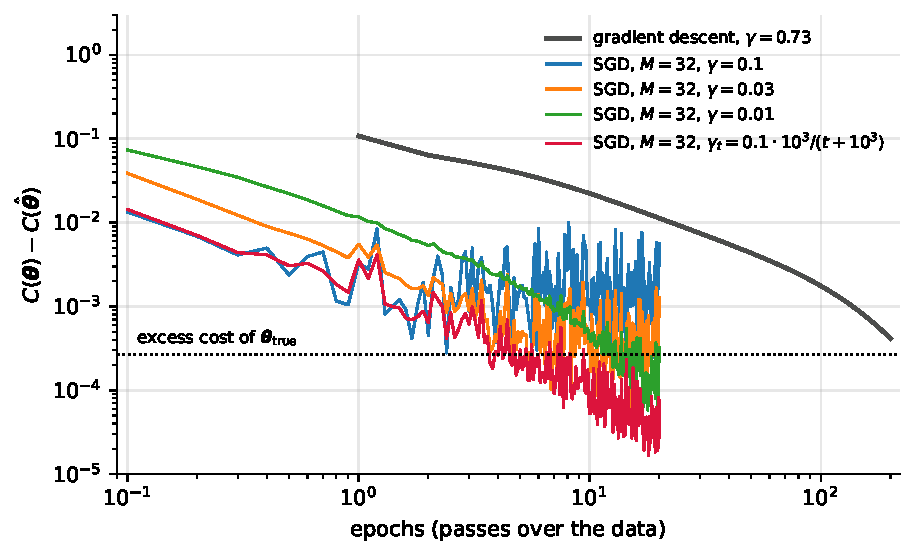
\includegraphics[width=0.8\textwidth]{BookFigures/chapter05_logistic_regression/logreg_sgd_vs_gd}
\caption{Excess cross entropy $C(\bm{\theta})-C(\hat{\bm{\theta}})$ against
passes over the data for the logistic regression problem of
Section~\ref{sec:logregsgdvsgd} ($n=50\,000$, $p=20$, $\kappa=173$).
Gradient descent uses the learning rate~(\ref{eq:5-gdstability}); the SGD
runs use minibatches of $M=32$, the cost being recorded ten times per
epoch, at three constant learning rates and with the decaying schedule
$\gamma_t=0.1\cdot10^{3}/(t+10^{3})$.  The dotted line is the excess cost of
the parameters that generated the data, about $p/(2n)$.  After a single epoch
every SGD run is where gradient descent is after twenty.  The constant-rate
runs then equilibrate in a cloud whose size grows with $\gamma$, as
Eq.~(\ref{eq:4-sgdcloud}) predicts, the smallest rate reaching within
twenty epochs the level gradient descent needs two hundred for; only the
decaying schedule continues downwards.}
\label{fig:5-sgdvsgd}
\end{figure}

Figure~\ref{fig:5-sgdvsgd} and the first block of the output below tell
the same story.  Gradient descent reduces the excess cost to
$1.1\times10^{-1}$ after one pass, $3.9\times10^{-2}$ after five,
$1.1\times10^{-2}$ after twenty and reaches $4.1\times10^{-4}$, about the
statistical floor, only after $200$ passes; the slow, steady slope is the
rate $(1-2/\kappa)^{k}$ of a problem with $\kappa=173$.  Stochastic gradient
descent with $M=32$ and $\gamma=0.01$ is at $1.8\times10^{-3}$ after five
passes and $3.2\times10^{-4}$ after twenty, so that five epochs of SGD are
worth about a hundred of gradient descent and twenty are worth two
hundred.  Since an epoch of either costs the same $4np$ operations, this is
a factor of ten to twenty in computation, obtained without tuning anything.
With the decaying schedule the excess is $3.0\times10^{-4}$ after five
epochs and $2.8\times10^{-5}$ after twenty -- an order of magnitude below
the floor, and still falling.  The larger constant rates show the other
side of the coin: $\gamma=0.1$ is fastest in the first epoch but then
oscillates in a band an order of magnitude wide, and the band for
$\gamma=0.03$ is narrower by about the ratio of the learning rates, as
Eq.~(\ref{eq:4-sgdcloud}) says it should be.  One more column of the output
deserves attention: the accuracy.  Gradient descent classifies $68.8\%$ of
the training points correctly after one pass, $74.3\%$ after five and
$76.1\%$ after twenty, while both SGD runs of the listing are at $76.7\%$
after twenty epochs, the accuracy of the true parameters.  The accuracy
saturates long before the cost does -- an excess cost of $10^{-3}$ already
gives an accuracy within half a percent of the best possible -- which is
why, for classification, a few epochs of SGD are usually all that is ever
run.

%......................................................................
\subsection{AdaGrad, RMSProp and Adam on the same problem}
\label{sec:logregadaptive}

\index{AdaGrad!logistic regression}\index{RMSProp!logistic regression}
\index{Adam!logistic regression}
The three adaptive methods of Sections~\ref{sec:adagrad} to~\ref{sec:adam}
replace the single learning rate of Eq.~(\ref{eq:5-sgdupdate}) by one per
parameter, obtained from a running average of the squared minibatch
gradients: AdaGrad accumulates the squares, Eq.~(\ref{eq:4-adagrad}),
RMSProp averages them with exponential forgetting,
Eq.~(\ref{eq:4-rmsprop}), and Adam adds a momentum-like average of the
gradient itself with bias corrections, Eq.~(\ref{eq:4-adam}).  All three
are the diagonally preconditioned iteration of Eq.~(\ref{eq:4-precond}),
and Chapter~\ref{chap:optim} drew two conclusions from that form: the
preconditioner equalises the curvature \emph{along the coordinate axes} and
therefore undoes any difference in the scales of the features, but it can
do nothing about curvature caused by correlation between them, which is not
diagonal.  Logistic regression lets us test both conclusions with one
switch, because the data of the previous subsection come standardised, and
we may unstandardise them.

Figure~\ref{fig:5-adaptive} shows the four stochastic methods -- plain SGD
and the three adaptive ones, minibatches of $32$ throughout -- and gradient
descent, first on the standardised features of Figure~\ref{fig:5-sgdvsgd}
and then on the same data with each feature column multiplied by a fixed
random factor between $0.1$ and $10$, the kind of disparity in units that
raw data carry.  For each method the constant learning rate was chosen from
a grid of five values a factor of $\sqrt{10}$ apart as the one with the
smallest mean excess cost over epochs $15$ to $20$; the listing below runs
the winners, and Table~\ref{tab:5-sgdcompare} collects the numbers.

\begin{figure}[htbp]
\centering
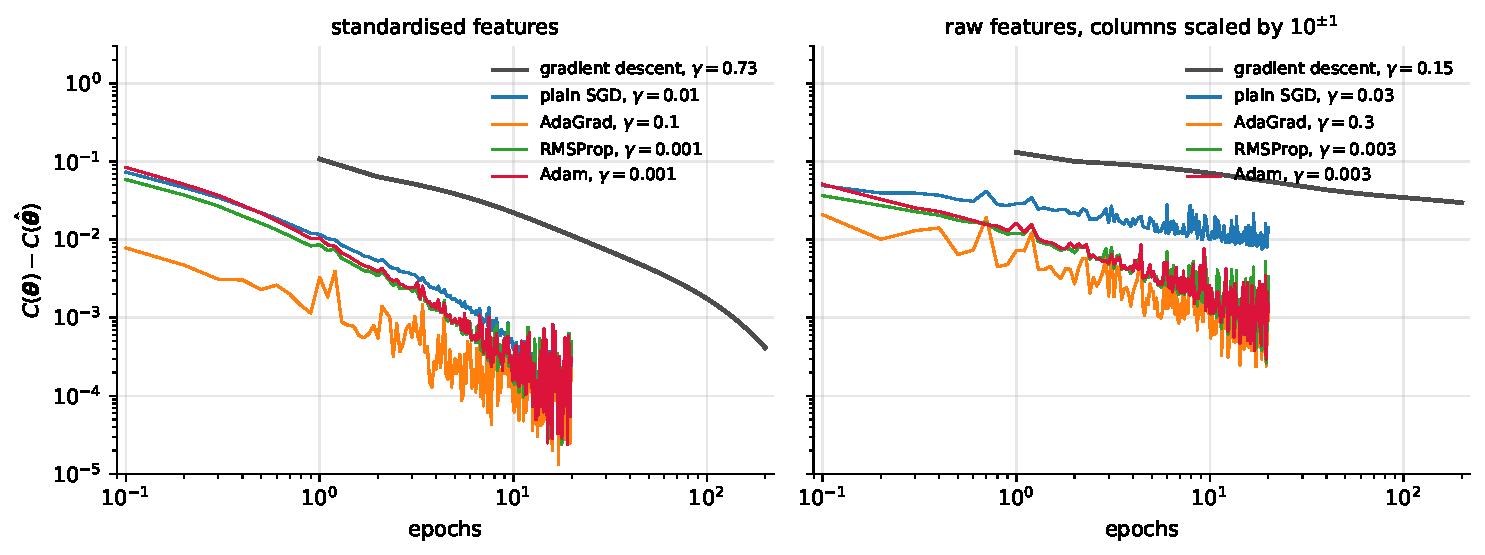
\includegraphics[width=0.98\textwidth]{BookFigures/chapter05_logistic_regression/logreg_adaptive}
\caption{Plain SGD, AdaGrad, RMSProp and Adam, all with $M=32$ and each at
the best of five constant learning rates, against gradient descent at the
learning rate~(\ref{eq:5-gdstability}), on the logistic regression problem
of Section~\ref{sec:logregsgdvsgd}.  Left: standardised features,
$\kappa=173$.  Right: the same data with each feature column multiplied by
a random factor between $0.1$ and $10$, which raises the condition number
of the Hessian at the optimum to $4.4\times10^{4}$ and the excess cost of
the two plain-gradient methods by nearly two orders of magnitude, while the
three adaptive methods lose less than one.  On standardised
features the four stochastic methods are indistinguishable after ten
epochs.}
\label{fig:5-adaptive}
\end{figure}

\begin{table}[htbp]
\centering
\caption{Excess cross entropy $C(\bm{\theta})-C(\hat{\bm{\theta}})$ and
training accuracy for the methods of Figure~\ref{fig:5-adaptive}, from the
output of the listing below.  Gradient descent is listed after $200$ epochs,
the stochastic methods after $20$; the column ``mean'' averages the excess
cost at the ends of epochs $15$ to $20$, which smooths the fluctuations of
the constant-rate runs.  The excess cost of the parameters that generated
the data is $2.7\times10^{-4}$ in both cases.}
\label{tab:5-sgdcompare}
\renewcommand{\arraystretch}{1.2}
\setlength{\tabcolsep}{6pt}
\begin{tabular}{lrrrr}
\toprule
\textbf{Method} & $\gamma$ & \textbf{excess, 5 epochs} & \textbf{mean, 15--20} & \textbf{accuracy}\\
\midrule
\multicolumn{5}{l}{\emph{standardised features, $\kappa=173$}}\\
gradient descent (200 epochs) & $0.73$  & $3.9\times10^{-2}$ & $4.1\times10^{-4}$ & $0.7671$\\
SGD                           & $0.01$  & $1.8\times10^{-3}$ & $1.9\times10^{-4}$ & $0.7666$\\
SGD, $\gamma_t=0.1\cdot10^{3}/(t+10^{3})$ & $0.1$ & $3.0\times10^{-4}$ & $5.1\times10^{-5}$ & $0.7671$\\
AdaGrad                       & $0.1$   & $3.0\times10^{-4}$ & $1.3\times10^{-4}$ & $0.7670$\\
RMSProp                       & $0.001$ & $9.4\times10^{-4}$ & $2.3\times10^{-4}$ & $0.7663$\\
Adam                          & $0.001$ & $9.7\times10^{-4}$ & $2.2\times10^{-4}$ & $0.7666$\\
\midrule
\multicolumn{5}{l}{\emph{raw features, $\kappa=4.4\times10^{4}$}}\\
gradient descent (200 epochs) & $0.15$  & $8.6\times10^{-2}$ & $3.0\times10^{-2}$ & $0.7471$\\
SGD                           & $0.03$  & $1.8\times10^{-2}$ & $1.2\times10^{-2}$ & $0.7585$\\
AdaGrad                       & $0.3$   & $2.2\times10^{-3}$ & $9.4\times10^{-4}$ & $0.7657$\\
RMSProp                       & $0.003$ & $3.6\times10^{-3}$ & $1.7\times10^{-3}$ & $0.7647$\\
Adam                          & $0.003$ & $3.3\times10^{-3}$ & $1.3\times10^{-3}$ & $0.7656$\\
\bottomrule
\end{tabular}
\end{table}

Three things stand out.  First, on standardised features the adaptive
methods bring nothing that plain SGD does not already have: after ten
epochs all four sit at the statistical floor, within a factor of two of
one another, and the ordering among them changes from epoch to epoch with
the noise.  The condition number $\kappa=173$ of this problem comes from the
correlation between the columns, not from their scales, and a diagonal
preconditioner cannot see it.  Second, on the raw features the picture
changes completely.  Gradient descent, forced by Eq.~(\ref{eq:5-gdstability})
to a learning rate five times smaller, is at an excess cost of
$3\times10^{-2}$ after $200$ epochs, worse than SGD on the standardised
data was after one; plain SGD is at $10^{-2}$ after twenty epochs, with a
training accuracy nearly a full percent below the optimum, and no constant learning
rate does better, since the step that suits the columns scaled by $10$
crawls on those scaled by $0.1$ and the reverse diverges.  The three
adaptive methods recover an order of magnitude of that loss, ending at
$10^{-3}$ with accuracies within a quarter of a percent of the optimum, because their
per-parameter learning rates absorb the column scales, as the scale
invariance of Section~\ref{sec:adaptive} says they must.  They do not
recover it all -- the remaining factor of five to ten against the
standardised case is the correlation, which survives rescaling.  Third, the
learning rates that work differ by two orders of magnitude between the
methods, and this is not a matter of tuning but of units: for plain SGD
$\gamma$ multiplies a gradient, while for RMSProp and Adam the update
$\gamma\,\bm{g}/\sqrt{\bm{v}}$ has the size of $\gamma$ itself in every
coordinate (Section~\ref{sec:adam}), so $\gamma$ is a step length in
parameter space and $10^{-3}$ is a sensible value; AdaGrad's ever-growing
accumulator shrinks its steps as $1/\sqrt{t}$, Eq.~(\ref{eq:4-adagradschedule}),
which is why it tolerates, and needs, a rate a hundred times larger.

The listing runs every method of Table~\ref{tab:5-sgdcompare}.  The
optimiser is the step function of Section~\ref{sec:adaptivecode}; the data
loop knows nothing about which method it is driving, and the gradient
function is the same for a minibatch as for the full data, which is all
that Eq.~(\ref{eq:5-minibatchgrad}) requires.

\begin{Python}{}
import numpy as np

def sigmoid(t):                          # the stable form of Section 5.7
    a = np.exp(-np.abs(t))
    return np.where(t >= 0, 1.0 / (1.0 + a), a / (1.0 + a))

def make_data(n=50_000, p=20, rho=0.9, seed=2026):
    """AR(1)-correlated standardised features, Bernoulli labels."""
    rng = np.random.default_rng(seed)
    z = rng.normal(size=(n, p - 1))
    xc = np.empty_like(z); xc[:, 0] = z[:, 0]
    for j in range(1, p - 1):
        xc[:, j] = rho * xc[:, j - 1] + np.sqrt(1 - rho**2) * z[:, j]
    xc = (xc - xc.mean(0)) / xc.std(0)
    X = np.column_stack([np.ones(n), xc])
    theta_true = 0.5 * rng.normal(size=p)
    y = (rng.random(n) < sigmoid(X @ theta_true)).astype(float)
    scales = np.concatenate([[1.0], 10.0**rng.uniform(-1, 1, p - 1)])
    return X, y, theta_true, scales     # scales: the "raw" units

def cost(X, y, theta):                   # mean cross entropy, Eq. (5.costmean)
    z = X @ theta
    return np.mean(np.logaddexp(0.0, z) - y * z)

def gradient(X, y, theta):               # Eq. (5.minibatchgrad), any rows
    return X.T @ (sigmoid(X @ theta) - y) / X.shape[0]

def optimiser_step(method, theta, g, state, t, gamma, rho=0.99,
                   beta1=0.9, beta2=0.999, eps=1e-8):
    """The step function of Section 4.12, without momentum."""
    if method == "plain":
        return theta - gamma * g
    if method == "adagrad":                                # Eq. (4.adagrad)
        state["r"] = r = state.get("r", 0.0) + g * g
        return theta - gamma * g / (np.sqrt(r) + eps)
    if method == "rmsprop":                                # Eq. (4.rmsprop)
        state["r"] = r = rho * state.get("r", 0.0) + (1 - rho) * g * g
        return theta - gamma * g / (np.sqrt(r) + eps)
    if method == "adam":                                   # Eq. (4.adam)
        state["m"] = m = beta1 * state.get("m", 0.0) + (1 - beta1) * g
        state["r"] = r = beta2 * state.get("r", 0.0) + (1 - beta2) * g * g
        m_hat, r_hat = m / (1 - beta1**t), r / (1 - beta2**t)
        return theta - gamma * m_hat / (np.sqrt(r_hat) + eps)

def train(X, y, method, gamma, M=None, epochs=20, t0=None, seed=1):
    """Minibatch loop, Eq. (5.sgdupdate); M=None is full-batch gradient
    descent.  Returns theta at the end of every epoch."""
    n, p = X.shape
    M = n if M is None else M
    rng = np.random.default_rng(seed)
    theta, state, t, history = np.zeros(p), {}, 0, []
    for epoch in range(epochs):
        idx = rng.permutation(n)
        for k in range(0, n, M):                   # one epoch = n/M updates
            t += 1
            gam = gamma if t0 is None else gamma * t0 / (t + t0)
            b = idx[k:k + M]
            g = gradient(X[b], y[b], theta)
            theta = optimiser_step(method, theta, g, state, t, gam)
        history.append(theta.copy())
    return history

def newton(X, y):                        # the reference, to machine precision
    theta = np.zeros(X.shape[1])
    for _ in range(50):
        pr = sigmoid(X @ theta)
        H = X.T @ ((pr * (1 - pr))[:, None] * X) / len(y)
        step = np.linalg.solve(H, X.T @ (pr - y) / len(y))
        theta -= step
        if np.linalg.norm(step) < 1e-12:
            break
    return theta

X, y, theta_true, scales = make_data()
settings = {                             # the winners of the learning-rate grid
    "standardised": [("SGD", "plain", 0.01), ("AdaGrad", "adagrad", 0.1),
                     ("RMSProp", "rmsprop", 0.001), ("Adam", "adam", 0.001)],
    "raw":          [("SGD", "plain", 0.03), ("AdaGrad", "adagrad", 0.3),
                     ("RMSProp", "rmsprop", 0.003), ("Adam", "adam", 0.003)]}
for label, Xd, th_true in (("standardised", X, theta_true),
                           ("raw", X * scales, theta_true / scales)):
    c_star = cost(Xd, y, newton(Xd, y))
    lam_max = np.linalg.eigvalsh(Xd.T @ Xd / len(y)).max()
    gamma_gd = 8.0 / lam_max                       # Eq. (5.gdstability)
    runs = [("GD, 200 epochs",
             dict(method="plain", gamma=gamma_gd, epochs=200))]
    runs += [(name, dict(method=m, gamma=gam, M=32))
             for name, m, gam in settings[label]]
    if label == "standardised":
        runs.insert(2, ("SGD, decaying",
                        dict(method="plain", gamma=0.1, M=32, t0=1e3)))
    print(f"{label} features: C* = {c_star:.5f}, "
          f"excess of theta_true {cost(Xd, y, th_true) - c_star:.1e}")
    print("  method           gamma    excess after 1 / 5 / 20 epochs"
          "   mean 15-20   accuracy")
    for name, kw in runs:
        hist = train(Xd, y, **kw)
        ex = np.array([cost(Xd, y, th) - c_star for th in hist])
        if len(ex) > 20:                       # gradient descent, 200 epochs
            e_last, e_mean = ex[199], ex[199]
        else:                                  # SGD: epoch 20, mean of 15-20
            e_last, e_mean = ex[19], ex[14:].mean()
        acc = np.mean((Xd @ hist[-1] > 0) == y)
        print(f"  {name:16s} {kw['gamma']:<7.3g}  {ex[0]:.1e} / {ex[4]:.1e} /"
              f" {e_last:.1e}      {e_mean:.1e}     {acc:.4f}")
\end{Python}

\begin{Python}{}
standardised features: C* = 0.47624, excess of theta_true 2.7e-04
  method           gamma    excess after 1 / 5 / 20 epochs   mean 15-20   accuracy
  GD, 200 epochs   0.734    1.1e-01 / 3.9e-02 / 4.1e-04      4.1e-04     0.7671
  SGD              0.01     1.2e-02 / 1.8e-03 / 3.2e-04      1.9e-04     0.7666
  SGD, decaying    0.1      3.6e-03 / 3.0e-04 / 2.8e-05      5.1e-05     0.7671
  AdaGrad          0.1      3.3e-03 / 3.0e-04 / 2.2e-04      1.3e-04     0.7670
  RMSProp          0.001    8.7e-03 / 9.4e-04 / 4.9e-04      2.3e-04     0.7663
  Adam             0.001    1.0e-02 / 9.7e-04 / 2.8e-04      2.2e-04     0.7666
raw features: C* = 0.47624, excess of theta_true 2.7e-04
  method           gamma    excess after 1 / 5 / 20 epochs   mean 15-20   accuracy
  GD, 200 epochs   0.148    1.3e-01 / 8.6e-02 / 3.0e-02      3.0e-02     0.7471
  SGD              0.03     2.9e-02 / 1.8e-02 / 1.4e-02      1.2e-02     0.7585
  AdaGrad          0.3      7.3e-03 / 2.2e-03 / 1.8e-03      9.4e-04     0.7657
  RMSProp          0.003    1.2e-02 / 3.6e-03 / 3.4e-03      1.7e-03     0.7647
  Adam             0.003    1.6e-02 / 3.3e-03 / 1.5e-03      1.3e-03     0.7656
\end{Python}

For the gradient-descent rows the column ``20 epochs'' holds the value
after $200$; the raw-feature reference $C^{*}$ is the standardised one, as
it must be, since rescaling the columns rescales the parameters and
nothing else, Section~\ref{sec:adaptive}.  The whole run takes a few
seconds, and changing the loss, the minibatch size or the optimiser is one
line each -- the loop is the one that will train every network in this
book.

\begin{notebox}
\textbf{Machine learning connection.}  The recommendation that falls out of
Table~\ref{tab:5-sgdcompare} is the one every practitioner follows:
standardise the features, as Section~\ref{sec:scalingintercept} advised on
other grounds, use minibatches, and reach for Adam or RMSProp when the
scales cannot be controlled -- in a neural network the inputs to the inner
layers are activations whose scales are set by the training itself, and
that is where the adaptive methods earn their keep.  For logistic
regression itself, \texttt{scikit-learn}'s \texttt{SGDClassifier} with
\texttt{loss="log\_loss"} is Eq.~(\ref{eq:5-sgdupdate}) with a decaying
learning rate and an $\ell_2$ penalty, and its \texttt{partial\_fit} method
is the minibatch loop of the listing exposed to the user; its default
\texttt{LogisticRegression} class, by contrast, is the Newton-type
\texttt{lbfgs} of Section~\ref{sec:logregoptim}, the right choice whenever
the data fit in memory and $p$ is modest.  The dividing line between the
two is the one drawn in Section~\ref{sec:newtoncompete}, now with a
measured example on each side of it.
\end{notebox}

%----------------------------------------------------------------------
\section{Other loss functions, and automatic differentiation}
\label{sec:logreglosses}

\index{loss function!for classification}\index{margin}
Everything so far has used the cross entropy, and Section~\ref{sec:crossentropy}
explained why it is the natural choice: it is the negative log-likelihood of
the Bernoulli model.  It is not, however, the only choice, and two of the most
important classifiers of the following chapters -- the support vector machine
of Chapter~\ref{chap:svm} and the boosting methods of
Chapter~\ref{chap:ensemble} -- are obtained from logistic regression by
changing nothing but the loss.  This section sets out the family, derives
what each member actually estimates, and then does something that would have
been tedious a chapter ago: fits all of them with one program, in which the
loss is an argument and no gradient is ever written down.  That is the
promise of Section~\ref{sec:autodiff} kept.

%......................................................................
\subsection{Margin-based losses}
\label{sec:marginlosses}

It is convenient to relabel the classes as $\tilde y_i=2y_i-1\in\{-1,+1\}$ and
to define the \emph{margin} of observation $i$,
\begin{equation}
  m_i = \tilde y_i\,t_i,
  \qquad t_i=\bm{x}_i^{T}\bm{\theta},
  \label{eq:5-margin}
\end{equation}
which is positive when the point is on the correct side of the decision
boundary $t=0$ and large when it is far from it.  The quantity we would like
to minimise is the number of misclassifications, the \emph{0--1 loss}
$\ell_{01}(m)=\mathbf{1}[m<0]$, but it is piecewise constant, so its
gradient is zero wherever it exists and no gradient method can move.  Every
practical classifier therefore minimises a \emph{surrogate}: a function
$\ell(m)$ that upper-bounds the 0--1 loss, decreases in $m$, and is smooth
enough or convex enough to optimise.  The cross entropy is one such surrogate.
Using $\sigma(-t)=1-\sigma(t)$, the per-observation cross entropy of
Eq.~(\ref{eq:5-crossentropycompact}) can be written as a function of the
margin alone,
\begin{equation}
  -y\log\sigma(t)-(1-y)\log[1-\sigma(t)]
   = -\log\sigma(\tilde y t) = \log\left(1+e^{-m}\right),
  \label{eq:5-logisticloss}
\end{equation}
the \emph{logistic loss}.  The other members of the family in common use are
collected in Table~\ref{tab:5-losses} and drawn in the left panel of
Fig.~\ref{fig:5-marginlosses}.

\begin{table}[htbp]
\centering
\small
\renewcommand{\arraystretch}{1.3}
\setlength{\tabcolsep}{4pt}
\begin{tabular}{@{}llccl@{}}
\toprule
\textbf{Loss} & $\ell(m)$ or $\ell(t,y)$ & convex in $t$ & $\sigma(t^{*})$ &
  \textbf{Where it is used}\\
\midrule
0--1 & $\mathbf{1}[m<0]$ & no & -- & the target, never optimised\\
logistic (cross entropy) & $\log(1+e^{-m})$ & yes & $\eta$ & logistic regression, networks\\
squared error (Brier) & $(y-\sigma(t))^{2}$ & no & $\eta$ & older networks, Brier score\\
hinge & $\max(0,1-m)$ & yes & sign only & support vector machines\\
squared hinge & $\max(0,1-m)^{2}$ & yes & $\sigma(2\eta-1)$ & $\ell_2$-SVM\\
exponential & $e^{-m}$ & yes & $\sigma(\tfrac12\log\frac{\eta}{1-\eta})$ & AdaBoost\\
focal & $-(1-p)^{\gamma}\log p$ & no & compressed & imbalanced data\\
\bottomrule
\end{tabular}
\caption{Loss functions for binary classification.  $m=\tilde y\,t$ is the
margin, $\eta=p(y=1\mid\bm{x})$ the true class probability, and $t^{*}$ the
value of the linear predictor that minimises the expected loss at a point,
Proposition~\ref{prop:5-bayeslosses}; for the focal loss $p$ denotes the
probability assigned to the correct class.  Only the losses whose $\sigma(t^{*})$
column reads $\eta$ estimate the class probability directly.}
\label{tab:5-losses}
\end{table}

\begin{figure}[htbp]
\centering
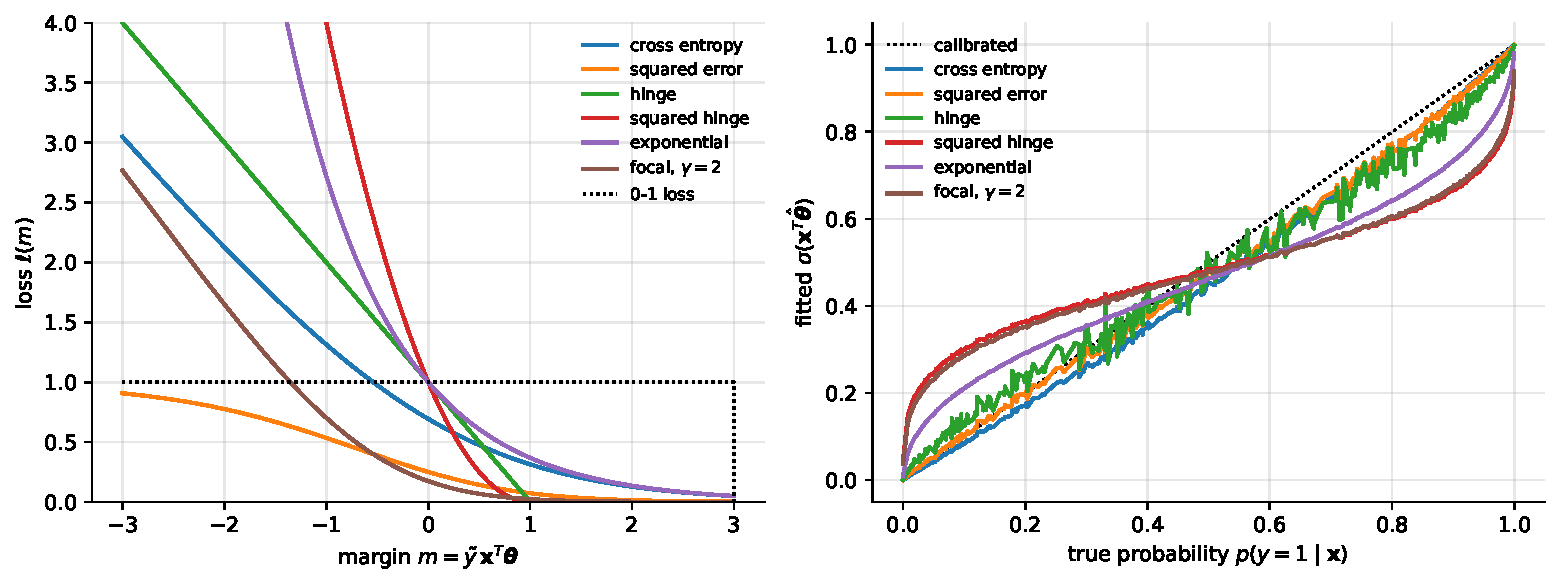
\includegraphics[width=0.98\textwidth]{BookFigures/chapter05_logistic_regression/margin_losses}
\caption{Left: the loss functions of Table~\ref{tab:5-losses} against the margin, for a point of class $\tilde y=+1$; the 0--1 loss is dotted.  Right: the probability $\sigma(\bm{x}^{T}\hat{\bm{\theta}})$ obtained by minimising each loss with a linear model on $400$ points drawn from a true logistic model, plotted against the true probability.  The cross entropy and the squared error follow the diagonal; the exponential loss recovers half the log-odds, so its curve is the diagonal compressed towards $\tfrac12$; the squared hinge and the focal loss are compressed further; the hinge loss does not estimate a probability at all.}
\label{fig:5-marginlosses}
\end{figure}

A few features of the picture are worth pointing out before the algebra.  All
the surrogates agree on the sign of what they want -- push the margin
positive -- and differ in how hard they push and where they stop.  The
hinge loss is exactly zero once $m\ge1$, so points comfortably on the right
side exert no force whatever; that is what will make support vectors in
Chapter~\ref{chap:svm}.  The logistic and exponential losses never reach zero
and keep rewarding larger margins, exponentially weakly in the first case and
linearly in the second; the exponential loss also punishes a large negative
margin \emph{exponentially} hard, which is the origin of AdaBoost's known
sensitivity to mislabelled points.  The squared error and the focal loss
flatten out for large negative margins, which is the vanishing-gradient
problem of the notebox in Section~\ref{sec:crossentropy} seen again: a
confidently wrong point produces almost no gradient.

%......................................................................
\subsection{What each loss estimates}
\label{sec:losscalibration}

\index{proper scoring rule}\index{calibration}
A loss function does two jobs.  It has to be minimised, which is a matter of
convexity and smoothness, and its minimiser has to mean something.  The
second question has a clean answer, because in the limit of infinite data the
fit at each $\bm{x}$ minimises the \emph{expected} loss there.  Fix a point
with true class probability $\eta=p(y=1\mid\bm{x})$ and ask which value of the
linear predictor $t$ minimises
\begin{equation}
  L(t) = \mathbb{E}_{y}\left[\ell(t,y)\right]
       = \eta\,\ell(t,1) + (1-\eta)\,\ell(t,0).
  \label{eq:5-expectedloss}
\end{equation}
For a margin loss $\ell(t,1)=\ell(t)$ and $\ell(t,0)=\ell(-t)$.  If the
minimiser $t^{*}$ has the sign of $2\eta-1$, the surrogate is
\emph{classification-calibrated}~\cite{bartlett2006}: minimising it recovers
the Bayes decision rule of the 0--1 loss.  If, further, $\sigma(t^{*})=\eta$
-- or some fixed, invertible function of $t^{*}$ equals $\eta$ -- the
surrogate is a \emph{proper scoring rule}~\cite{brier1950,gneiting2007} and the
model's output can be read as a probability.

\begin{proposition}[Pointwise minimisers of the classification losses]
\label{prop:5-bayeslosses}
For $0<\eta<1$ the minimiser of Eq.~(\ref{eq:5-expectedloss}) is
\begin{align}
  \text{logistic:}\quad
    &t^{*}=\log\frac{\eta}{1-\eta},
    &&\sigma(t^{*})=\eta;
  \label{eq:5-bayeslogistic}\\
  \text{squared error:}\quad
    &\sigma(t^{*})=\eta;
  \label{eq:5-bayessquared}\\
  \text{exponential:}\quad
    &t^{*}=\tfrac12\log\frac{\eta}{1-\eta},
    &&\sigma(2t^{*})=\eta;
  \label{eq:5-bayesexp}\\
  \text{squared hinge:}\quad
    &t^{*}=2\eta-1;
  \label{eq:5-bayessqhinge}\\
  \text{hinge:}\quad
    &t^{*}=\mathrm{sign}(2\eta-1).
  \label{eq:5-bayeshinge}
\end{align}
All five are classification-calibrated.  The logistic and squared-error
losses are proper; the exponential and squared-hinge losses determine $\eta$
through $\sigma(2t^{*})$ and $(t^{*}+1)/2$ respectively; the hinge loss
carries no information about $\eta$ beyond its sign.
\end{proposition}

\begin{proof}
Each is a one-variable minimisation.  For the logistic loss,
$L(t)=\eta\log(1+e^{-t})+(1-\eta)\log(1+e^{t})$ and
$L'(t)=-\eta(1-\sigma(t))+(1-\eta)\sigma(t)=\sigma(t)-\eta$, which vanishes
exactly at $\sigma(t^{*})=\eta$; $L''=\sigma(1-\sigma)>0$, so it is the
minimum.  For the squared error,
$L(t)=\eta(1-\sigma)^{2}+(1-\eta)\sigma^{2}$ with $\sigma=\sigma(t)$, and
$L'(t)=2(\sigma-\eta)\,\sigma'(t)$; since $\sigma'>0$ the only stationary
point is again $\sigma(t^{*})=\eta$, and $L\to\eta$ or $1-\eta$ at
$t\to\mp\infty$, both larger than the value $\eta(1-\eta)$ at the stationary
point, so it is the global minimum although $L$ is not convex.  For the
exponential loss $L(t)=\eta e^{-t}+(1-\eta)e^{t}$, $L'(t)=-\eta e^{-t}
+(1-\eta)e^{t}=0$ gives $e^{2t^{*}}=\eta/(1-\eta)$, and
$\sigma(2t^{*})=e^{2t^{*}}/(1+e^{2t^{*}})=\eta$.  For the squared hinge the
minimiser lies in $[-1,1]$, where both hinges are active,
$L(t)=\eta(1-t)^{2}+(1-\eta)(1+t)^{2}$ and $L'(t)=-2\eta(1-t)+2(1-\eta)(1+t)
=2(t-(2\eta-1))$.  For the hinge, $L(t)=\eta\max(0,1-t)+(1-\eta)\max(0,1+t)$
is piecewise linear with slope $-\eta+(1-\eta)=1-2\eta$ on $[-1,1]$, slope
$1-\eta>0$ for $t>1$ and slope $-\eta<0$ for $t<-1$; it is therefore
minimised at $t=1$ if $\eta>\tfrac12$ and at $t=-1$ if $\eta<\tfrac12$, and
the value at the minimum, $2\min(\eta,1-\eta)$, depends on $\eta$ but its
location does not.  In every case $\mathrm{sign}(t^{*})=\mathrm{sign}(2\eta-1)$.
\qed
\end{proof}

The proposition is what the right panel of Fig.~\ref{fig:5-marginlosses}
shows empirically, and it explains a common misuse.  A support vector machine
does not produce probabilities, and passing its decision function through a
sigmoid produces numbers that are systematically too close to $\tfrac12$ --
which is why \texttt{scikit-learn} fits a separate logistic regression on top
of the SVM output when probabilities are requested (Platt scaling).  A model
trained with the exponential loss must be read through $\sigma(2t)$, not
$\sigma(t)$; that is why the AdaBoost of Chapter~\ref{chap:ensemble} outputs
half the log-odds.  And the focal loss~\cite{lin2017},
\begin{equation}
  \ell_{\mathrm{focal}}(t,y)
   = -y\,(1-p)^{\gamma}\log p - (1-y)\,p^{\gamma}\log(1-p),
  \qquad p=\sigma(t),\ \gamma\ge0,
  \label{eq:5-focal}
\end{equation}
which multiplies each cross-entropy term by a factor that vanishes for
well-classified points and thereby concentrates the gradient on the hard and
the rare ones, is deliberately \emph{not} proper: its minimiser is pushed
towards $\tfrac12$ (Exercise at the end of the chapter), so a detector trained
with it must be recalibrated before its scores are read as probabilities.
The cross entropy is the only member of the family that is convex, proper,
and free of the vanishing-gradient defect, and that is the whole case for it;
but each of the others buys something in exchange, and the following code
makes it possible to see what without deriving a single derivative.

%......................................................................
\subsection{One program for every loss}
\label{sec:losscode}

\index{JAX!logistic regression}
The class of Section~\ref{sec:logregcode} hard-wired the cross-entropy
gradient~(\ref{eq:5-gradient}).  With automatic differentiation the loss
becomes a plain Python function of the linear predictor and the label, the
cost is its mean over the data plus the penalty of Eq.~(\ref{eq:5-penalised}),
and JAX supplies the gradient -- and, if wanted, the Hessian -- of whatever
we wrote.  Trying a new loss means writing one line.

\begin{Python}{}
import jax
jax.config.update("jax_enable_x64", True)
import jax.numpy as jnp
import numpy as np
from jax import grad, jit, hessian
from jax.nn import sigmoid, softplus, log_sigmoid

# Every loss is a function of the linear predictor t = x^T theta and the label
# y in {0, 1}, evaluated pointwise; softplus(t) = log(1 + e^t) is the stable
# form of Eq. (5.crossentropycompact), log_sigmoid(t) = log sigma(t).
def cross_entropy(t, y):
    return softplus(t) - y * t                          # Eq. (5.logisticloss)

def squared_error(t, y):
    return (y - sigmoid(t))**2                          # the Brier score

def hinge(t, y):
    return jnp.maximum(0.0, 1.0 - (2*y - 1) * t)        # margin m = (2y-1) t

def squared_hinge(t, y):
    return jnp.maximum(0.0, 1.0 - (2*y - 1) * t)**2

def exponential(t, y):
    return jnp.exp(-(2*y - 1) * t)

def focal(t, y, gamma=2.0):                             # Eq. (5.focal)
    p = sigmoid(t)
    return -(y * (1 - p)**gamma * log_sigmoid(t)
             + (1 - y) * p**gamma * log_sigmoid(-t))

LOSSES = {"cross entropy": cross_entropy, "squared error": squared_error,
          "hinge": hinge, "squared hinge": squared_hinge,
          "exponential": exponential, "focal (gamma=2)": focal}

def cost(theta, X, y, loss, lmbda=0.0):
    """Mean loss over the data plus an l2 penalty that spares the intercept."""
    return jnp.mean(loss(X @ theta, y)) + lmbda * jnp.sum(theta[1:]**2)

def fit(loss, X, y, gamma=0.5, epochs=3000, lmbda=0.0):
    """Gradient descent, Eq. (5.gd), with the gradient supplied by JAX."""
    c = lambda th: cost(th, X, y, loss, lmbda)
    step = jit(lambda th: th - gamma * grad(c)(th))
    theta = jnp.zeros(X.shape[1])
    for _ in range(epochs):
        theta = step(theta)
    return theta

def newton(loss, X, y, iters=10, lmbda=1e-8):
    """Newton-Raphson, Eq. (5.newtonabstract), with the Hessian from JAX."""
    c = lambda th: cost(th, X, y, loss, lmbda)
    g, H = jit(grad(c)), jit(hessian(c))
    theta = jnp.zeros(X.shape[1])
    for _ in range(iters):
        theta = theta - jnp.linalg.solve(H(theta), g(theta))
    return theta
\end{Python}

Before using it on anything, we check the machinery against the hand-derived
results of Section~\ref{sec:logreggradient}: the automatic gradient of the
cross entropy must be $-\bm{X}^{T}(\bm{y}-\bm{p})/n$ and its automatic
Hessian must be $\bm{X}^{T}\bm{W}\bm{X}/n$.  The data are drawn from a
\emph{true} logistic model, so that we can afterwards ask not only whether
each loss classifies well but whether it estimates the right probabilities.

\begin{Python}{}
rng = np.random.default_rng(2024)
n = 400
X = jnp.asarray(np.c_[np.ones(n), rng.normal(size=(n, 2))])
theta_true = jnp.array([0.5, 2.0, -1.0])
p_true = sigmoid(X @ theta_true)                       # the truth we try to recover
y = jnp.asarray((rng.random(n) < np.asarray(p_true)).astype(float))

theta0 = jnp.array([0.1, -0.3, 0.2])
g_ad = grad(cost)(theta0, X, y, cross_entropy)
g_hand = -X.T @ (y - sigmoid(X @ theta0)) / n                 # Eq. (5.gradient)
print("gradient: max |AD - hand| =", float(jnp.max(jnp.abs(g_ad - g_hand))))

p0 = sigmoid(X @ theta0)
H_ad = hessian(cost)(theta0, X, y, cross_entropy)
H_hand = X.T @ ((p0 * (1 - p0))[:, None] * X) / n              # Eq. (5.hessian)
print("Hessian:  max |AD - hand| =", float(jnp.max(jnp.abs(H_ad - H_hand))))

print("Newton :", newton(cross_entropy, X, y))
print("GD     :", fit(cross_entropy, X, y))
\end{Python}

\begin{Python}{}
gradient: max |AD - hand| = 2.220446049250313e-16
Hessian:  max |AD - hand| = 3.0531133177191805e-16
Newton : [ 0.26067864  1.93734364 -1.00125907]
GD     : [ 0.26067869  1.93734439 -1.00125944]
\end{Python}

Both derivatives agree with Eqs.~(\ref{eq:5-gradient}) and (\ref{eq:5-hessian})
to rounding, and Newton's method built from \texttt{jax.hessian} lands in ten
iterations where three thousand steps of gradient descent land, the two
differing in the seventh digit only through the tiny ridge term that keeps
the Hessian invertible.  Now the loop that
motivated the section:

\begin{Python}{}
def evaluate(theta):
    p = sigmoid(X @ theta)
    accuracy = float(jnp.mean((p > 0.5) == (y > 0.5)))
    calibration = float(jnp.mean(jnp.abs(p - p_true)))    # mean |p_hat - p_true|
    return accuracy, calibration

print(f"{'loss':16s} {'theta':26s} accuracy   mean |p_hat - p_true|")
for name, loss in LOSSES.items():
    theta = fit(loss, X, y)
    acc, cal = evaluate(theta)
    print(f"{name:16s} {np.array2string(np.asarray(theta), precision=2):26s}"
          f" {acc:.3f}      {cal:.3f}")
print("true            ", np.asarray(theta_true))
\end{Python}

\begin{Python}{}
loss             theta                      accuracy   mean |p_hat - p_true|
cross entropy    [ 0.26  1.94 -1.  ]        0.790      0.032
squared error    [ 0.32  1.82 -0.97]        0.790      0.024
hinge            [ 0.28  1.53 -0.89]        0.792      0.043
squared hinge    [ 0.1   0.69 -0.36]        0.795      0.156
exponential      [ 0.11  1.06 -0.53]        0.780      0.103
focal (gamma=2)  [ 0.09  0.74 -0.38]        0.782      0.149
true             [ 0.5  2.  -1. ]
\end{Python}

The accuracies are all within a percent of one another, and of the Bayes rate
of $0.79$ for this problem: every loss in the table is classification-calibrated,
as Proposition~\ref{prop:5-bayeslosses} says, and all of them find essentially
the same decision boundary.  The probabilities are another matter, and the
last column is Proposition~\ref{prop:5-bayeslosses} in numbers.  The two
proper losses recover the true parameters up to sampling error.  The
exponential loss returns $(0.11,1.06,-0.53)$, which is the true vector halved
-- Eq.~(\ref{eq:5-bayesexp}), $t^{*}=\tfrac12\log[\eta/(1-\eta)]$ -- and its
probabilities are correct once read through $\sigma(2t)$.  The squared hinge
and the focal loss compress the parameters by a factor of about three and
their $\sigma(t)$ is badly miscalibrated, while their accuracy is unharmed.
Nothing about these conclusions required a derivative, and the reader can now
add a loss to the dictionary -- an asymmetric one that penalises false
negatives more than false positives, a class-weighted cross entropy, a
Huberised hinge -- and have the answer in seconds.

\begin{notebox}
\textbf{Machine learning connection.}  The pattern of this section is how
loss functions are actually developed.  A practitioner writes the loss as a
few lines of framework code, lets the framework differentiate it, and judges
the result empirically; the theoretical questions -- is it convex, is it
proper, is it classification-calibrated -- are asked afterwards, and often
answered by exactly the pointwise argument of
Proposition~\ref{prop:5-bayeslosses}.  Every framework in the later chapters
(\texttt{PyTorch}, \texttt{TensorFlow}, \texttt{JAX}) offers the losses of
Table~\ref{tab:5-losses} as library functions, but nothing in them is
special: \texttt{torch.nn.BCEWithLogitsLoss} is \texttt{softplus(t) - y*t},
and a loss the library does not offer is one line away.  The one practical
rule is the one used above: write losses in terms of the logit $t$ and the
stable primitives \texttt{softplus} and \texttt{log\_sigmoid}, never in terms
of $\log\sigma(t)$ computed literally, for the reasons of
Section~\ref{sec:logregoptim}.
\end{notebox}

%----------------------------------------------------------------------
\section{Kernel logistic regression}
\label{sec:kernellogreg}

\index{kernel logistic regression}\index{logistic regression!kernel}
Logistic regression produces a linear decision boundary, and
Section~\ref{sec:kernelmethods} showed how to remove that restriction from
Ridge regression without ever constructing the enlarged feature space.  The
same construction applies here, and it applies for the same reason: by
Theorem~\ref{thm:3-representer} the reason had nothing to do with the squared
error.

%......................................................................
\subsection{The problem, and what the representer theorem gives}
\label{sec:klogregsetup}

Replace the linear predictor $\bm{x}^{T}\bm{\theta}$ by a function
$f\in\mathcal{H}$, the reproducing kernel Hilbert space of a kernel $k$, and
penalise its norm:
\begin{equation}
  \min_{f\in\mathcal{H}}\left\{
    -\sum_{i=1}^{n}\Big[y_i\ln p_i + (1-y_i)\ln(1-p_i)\Big]
    + \frac{\lambda}{2}\left\|f\right\|_{\mathcal{H}}^{2}\right\},
  \qquad
  p_i = \sigma\!\left(f(\bm{x}_i)\right),
  \label{eq:5-klogregproblem}
\end{equation}
with $\sigma$ the logistic function~(\ref{eq:5-sigmoid}) and $y_i\in\{0,1\}$.
The data-fitting term is the cross entropy~(\ref{eq:5-crossentropy}) with
$\bm{x}_i^{T}\bm{\theta}$ replaced by $f(\bm{x}_i)$, and the penalty is the
$\ell_2$ penalty of Section~\ref{sec:logregpenalty} measured in $\mathcal{H}$
rather than in $\mathbb{R}^{p}$.

Theorem~\ref{thm:3-representer} applies immediately: the loss depends on $f$
only through its values at the training points, and
$\Omega(t)=\tfrac{\lambda}{2}t^{2}$ is strictly increasing.  The minimiser is
therefore
\begin{equation}
  f(\cdot) = \sum_{j=1}^{n}\alpha_j\,k\!\left(\bm{x}_j,\cdot\right),
  \qquad\text{so that}\qquad
  \bm{f} = \bm{K}\bm{\alpha}
  \quad\text{and}\quad
  \left\|f\right\|_{\mathcal{H}}^{2}
   = \bm{\alpha}^{T}\bm{K}\bm{\alpha},
  \label{eq:5-krepresenter}
\end{equation}
the second identity because
$\|f\|^{2}=\sum_{ij}\alpha_i\alpha_j\langle k(\bm{x}_i,\cdot),
k(\bm{x}_j,\cdot)\rangle$, which is $\sum_{ij}\alpha_i\alpha_jK_{ij}$.  The
infinite-dimensional problem has become the $n$-dimensional one
\begin{equation}
  \boxed{\;
  C(\bm{\alpha}) =
    -\sum_{i=1}^{n}\Big[y_i\ln p_i+(1-y_i)\ln(1-p_i)\Big]
    + \frac{\lambda}{2}\,\bm{\alpha}^{T}\bm{K}\bm{\alpha},
  \qquad
  \bm{p} = \sigma\!\left(\bm{K}\bm{\alpha}\right). \;}
  \label{eq:5-kcost}
\end{equation}

%......................................................................
\subsection{Gradient, Hessian and kernel IRLS}
\label{sec:kirls}

The derivatives are obtained from Section~\ref{sec:logreggradient} by the
substitution $\bm{X}\rightarrow\bm{K}$, which is the whole of the work: the
chain rule sees $\bm{K}\bm{\alpha}$ exactly as it saw $\bm{X}\bm{\theta}$.
Differentiating Eq.~(\ref{eq:5-kcost}) and using
Eq.~(\ref{eq:1-dquadsym}) for the penalty,
\begin{equation}
  \frac{\partial C}{\partial\bm{\alpha}}
   = -\bm{K}\left(\bm{y}-\bm{p}\right) + \lambda\bm{K}\bm{\alpha}
   = \bm{K}\Big[\left(\bm{p}-\bm{y}\right)+\lambda\bm{\alpha}\Big],
  \label{eq:5-kgradient}
\end{equation}
to be compared with Eq.~(\ref{eq:5-gradient}), and
\begin{equation}
  \frac{\partial^{2}C}
       {\partial\bm{\alpha}\,\partial\bm{\alpha}^{T}}
   = \bm{K}\bm{W}\bm{K} + \lambda\bm{K},
  \label{eq:5-khessian}
\end{equation}
with $\bm{W}$ the same diagonal matrix~(\ref{eq:5-Wmatrix}) of weights
$p_i(1-p_i)$.  Since $\bm{K}$ is positive semi-definite, so is
Eq.~(\ref{eq:5-khessian}) by the argument of Eq.~(\ref{eq:5-convexproof}), and
the problem is convex; for $\lambda>0$ and $\bm{K}$ positive definite it is
strictly convex, so the minimiser is unique.

Newton's method now takes a form worth deriving, because it turns out to be the
exact analogue of the iteratively reweighted least squares of
Eq.~(\ref{eq:5-irls}).  Assume $\bm{K}$ invertible and factor it out of
Eq.~(\ref{eq:5-khessian}) on the left,
$\bm{K}\bm{W}\bm{K}+\lambda\bm{K}=\bm{K}(\bm{W}\bm{K}+\lambda\bm{I})$.  The
Newton step $\bm{\Delta}=-\bm{H}^{-1}\bm{g}$ is then
\begin{equation}
  \bm{\Delta}
   = -\left(\bm{W}\bm{K}+\lambda\bm{I}\right)^{-1}\bm{K}^{-1}
      \bm{K}\Big[(\bm{p}-\bm{y})+\lambda\bm{\alpha}\Big]
   = \left(\bm{W}\bm{K}+\lambda\bm{I}\right)^{-1}
     \Big[(\bm{y}-\bm{p})-\lambda\bm{\alpha}\Big],
  \label{eq:5-knewtonstep}
\end{equation}
the inverse Gram matrices cancelling.  Adding $\bm{\alpha}$ and collecting,
\begin{equation}
  \bm{\alpha}+\bm{\Delta}
   = \left(\bm{W}\bm{K}+\lambda\bm{I}\right)^{-1}
     \Big[\bm{W}\bm{K}\bm{\alpha}+(\bm{y}-\bm{p})\Big]
   = \left(\bm{W}\bm{K}+\lambda\bm{I}\right)^{-1}\bm{W}\bm{z},
  \label{eq:5-kirlsstep}
\end{equation}
where the \emph{working response}
\begin{equation}
  \bm{z} = \bm{K}\bm{\alpha}+\bm{W}^{-1}\left(\bm{y}-\bm{p}\right)
  \label{eq:5-kworking}
\end{equation}
is the adjusted response defined just above Eq.~(\ref{eq:5-irls}), with $\bm{X}\bm{\theta}$ replaced by
$\bm{K}\bm{\alpha}$.  Multiplying Eq.~(\ref{eq:5-kirlsstep}) through by
$\bm{W}^{-1}$ inside the inverse gives the form to remember,
\begin{equation}
  \boxed{\;
  \bm{\alpha} \;\leftarrow\;
    \left(\bm{K}+\lambda\bm{W}^{-1}\right)^{-1}\bm{z} . \;}
  \label{eq:5-kirls}
\end{equation}

Compare Eq.~(\ref{eq:5-kirls}) with the kernel ridge
regression~(\ref{eq:3-krr}), $\bm{\alpha}=(\bm{K}+\lambda\bm{I})^{-1}\bm{y}$.
They differ in two places only: the targets $\bm{y}$ have become the working
response $\bm{z}$, and the uniform penalty $\lambda\bm{I}$ has become the
per-observation penalty $\lambda\bm{W}^{-1}$, which is small where the model is
uncertain and large where it is confident.  \emph{Kernel logistic regression is
iteratively reweighted kernel ridge regression}, exactly as ordinary logistic
regression is iteratively reweighted least squares.  The parallel of
Section~\ref{sec:logregoptim} is complete, and it is not a coincidence but a
consequence of Theorem~\ref{thm:3-representer}: the same substitution that
turned least squares into kernel ridge regression turns each reweighted step
into a reweighted kernel step.

\begin{Python}{}
import numpy as np

def kernel_irls(K, y, lmbda, n_iter=100, tol=1e-13, jitter=1e-12):
    """Kernel logistic regression by Newton's method, Eq. (5.kirls).

    Each iteration is a kernel ridge regression, Eq. (3.krr), on the working
    response z with the per-observation penalty lambda / W_ii.
    """
    n = len(y)
    alpha = np.zeros(n)
    for _ in range(n_iter):
        f = K @ alpha
        p = sigmoid(f)
        w = np.maximum(p * (1.0 - p), 1e-10)          # W_ii, Eq. (5.Wmatrix)
        z = f + (y - p) / w                           # Eq. (5.kworking)
        new = np.linalg.solve(K + lmbda * np.diag(1.0 / w)
                              + jitter * np.eye(n), z)
        if np.linalg.norm(new - alpha) < tol:
            return new
        alpha = new
    return alpha


def kernel_logistic_predict(alpha, Xtrain, Xnew, gamma):
    """p(y=1|x) = sigma(sum_j alpha_j k(x_j, x))."""
    return sigmoid(gaussian_kernel(Xnew, Xtrain, gamma) @ alpha)
\end{Python}

The \verb!jitter! is there because $\bm{K}$ for a Gaussian kernel is positive
definite in exact arithmetic and can be numerically singular when two training
points nearly coincide; adding $10^{-12}$ to the diagonal is the standard
remedy and changes nothing that matters.

%......................................................................
\subsection{The method, verified}
\label{sec:klogregverify}

The test problem is one that no linear boundary can solve at all: $120$ points
in the plane, labelled by whether they fall inside a disc, with five per cent of
the labels flipped.  Newton's method on Eq.~(\ref{eq:5-kirls}) with a Gaussian
kernel converges in six iterations, and the step lengths show the quadratic
rate of Section~\ref{sec:logregoptim} unmistakably:

\begin{Python}{}
    iteration        cost          ||delta alpha||
            1    56.8201866189          3.602e+00
            2    56.4403059843          2.888e-01
            3    56.4394190411          1.438e-02
            4    56.4394190342          3.825e-05
            5    56.4394190342          3.059e-10
            6    56.4394190342          2.018e-15
\end{Python}

Each step length is roughly the square of the one before once the iterate is
close, which is what distinguishes Newton's method from the linearly convergent
gradient descent of Chapter~\ref{chap:optim}.  Plain gradient descent on the
same objective reaches the same minimum, more slowly: it agrees with the Newton
solution to $9.1\times10^{-5}$ in the fitted function, which is its own
convergence tolerance and not a disagreement about the answer.

The more searching test is against the primal problem.  With the quadratic
kernel $(\bm{x}^{T}\bm{x}'+1)^{2}$ the feature map is only six-dimensional, so
the same fit can be obtained by ordinary penalised logistic regression in that
map and the two compared:

\begin{Python}{}
  max |k(x,x') - phi(x).phi(x')|: 4.263e-14
  max |f_kernel(x) - f_primal(x)| on 400 test points: 6.004e-13
  ||theta_primal||^2 = 13.2542532295,   alpha^T K alpha = 13.2542532295

  scikit-learn in the same map, C = 1/lambda:
    max |theta_ours - theta_sklearn| : 9.498e-09
    max |f_ours - f_sklearn| on test : 7.232e-08
\end{Python}

The third line is the one to notice.  The primal penalty
$\|\bm{\theta}\|_2^{2}$ and the dual penalty
$\bm{\alpha}^{T}\bm{K}\bm{\alpha}$ agree to ten digits because they are the
same number written twice: both are $\|f\|_{\mathcal{H}}^{2}$, the squared norm
of one function in one space.  Note also the conversion to
\texttt{scikit-learn}'s convention, $C=1/\lambda$, warned about in
Section~\ref{sec:logregpenalty}; with it, three independent implementations
agree to the tolerance of the least accurate.

%......................................................................
\subsection{What the coefficients are}
\label{sec:kalpharesidual}

Setting Eq.~(\ref{eq:5-kgradient}) to zero gives a fact about kernel logistic
regression that is easy to miss and explains a good deal.

\begin{proposition}[The coefficients are the residuals]
\label{prop:5-kalpharesidual}
If $\bm{K}$ is invertible, the minimiser of Eq.~(\ref{eq:5-kcost}) satisfies
\begin{equation}
  \alpha_i = \frac{y_i-p_i}{\lambda},
  \qquad i=1,\dots,n .
  \label{eq:5-kalpharesidual}
\end{equation}
\end{proposition}

\begin{proof}
Stationarity is
$\bm{K}[(\bm{p}-\bm{y})+\lambda\bm{\alpha}]=\bm{0}$ by
Eq.~(\ref{eq:5-kgradient}).  Multiplying by $\bm{K}^{-1}$ gives
$\lambda\bm{\alpha}=\bm{y}-\bm{p}$.
\qed
\end{proof}

The weight a training point carries in the fitted
function~(\ref{eq:5-krepresenter}) is its own residual divided by the penalty.
Points the model already predicts correctly and confidently have small
residuals and contribute little; points it gets wrong contribute much.  But
$p_i$ is a logistic probability and lies strictly between zero and one, so the
residual $y_i-p_i$ is \emph{never exactly zero}: every training point
contributes something, and $\bm{\alpha}$ is dense.

\begin{Python}{}
   lambda   max |alpha - (y-p)/lambda|   non-zero alpha of 120   |alpha|_min
     0.10                   1.471e-11                 120   2.065e-02
     1.00                   1.477e-13                 120   6.360e-02
    10.00                   1.422e-15                 120   3.472e-02
\end{Python}

This is the practical drawback of the method and the reason it is less used
than its two neighbours.  Prediction costs $n$ kernel evaluations no matter
how easy the problem is, where a support vector machine on the same data would
retain a fraction of the points.  Section~\ref{sec:threelosses} shows that this
contrast is not an accident of the two algorithms but a theorem about their
losses, and that Eq.~(\ref{eq:5-kalpharesidual}) is one instance of a formula
covering all three of the kernel methods in this book.

\begin{notebox}
\textbf{Machine learning connection.}  What kernel logistic regression buys
over a support vector machine is a calibrated probability.  The output of
Eq.~(\ref{eq:5-krepresenter}) passed through the sigmoid is an estimate of
$p(y=1\mid\bm{x})$ obtained by maximising a likelihood, so it can be
thresholded at a cost-sensitive value, combined with other probabilities, or
fed to a decision rule -- all of which the signed distance produced by
Eq.~(\ref{eq:6-kernelclassify}) cannot support without an extra calibration
step fitted on held-out data.  Against that stands the dense $\bm{\alpha}$ of
Proposition~\ref{prop:5-kalpharesidual} and the $\bigO(n^{3})$ cost of each
Newton step.  The choice between them is the usual one in this book: a
probability, or a sparse representation, but not both from the same fit.
\end{notebox}

%......................................................................
\subsection{The penalty, measured}
\label{sec:klogregpenalty}

Everything Section~\ref{sec:logregpenalty} said about the penalty holds here,
with one addition: the kernel supplies enough flexibility to interpolate the
training data exactly, so the penalty is no longer optional.  Running the same
fit across six decades:

\begin{Python}{}
   lambda    train accuracy   test accuracy   alpha^T K alpha
     0.001           0.9500          0.9300         5027.0188
     0.010           0.9417          0.9275          696.1591
     0.100           0.9500          0.9375          144.9844
     1.000           0.9333          0.9400           22.4656
    10.000           0.8750          0.9150            1.0326
   100.000           0.8667          0.8700            0.0146
\end{Python}

The best test accuracy is at $\lambda=1$, in the interior, with the norm of the
fitted function falling by five orders of magnitude across the range.  At
$\lambda=10^{-3}$ the model is reproducing the five per cent of deliberately
flipped labels and pays for it on the test set; at $\lambda=100$ it has been
flattened towards a constant.  This is Eq.~(\ref{eq:2-biasvariance}) once
more, and it is why the kernel and the penalty must be chosen together by the
cross-validation of Section~\ref{sec:crossvalidation} and never by the
training error.

%----------------------------------------------------------------------
\section{Measuring the quality of a classifier}
\label{sec:classmetrics}

\index{confusion matrix}\index{accuracy}\index{precision}\index{recall}
The mean squared error and $R^{2}$ of Section~\ref{sec:metrics} are
meaningless for a classifier.  We need measures appropriate to discrete
outcomes, and it turns out that no single number will do.

\paragraph{The confusion matrix.}
Everything starts here.  For two classes, cross-tabulating the true label
against the predicted one gives four counts:
\begin{equation}
  \begin{array}{c|cc}
     & \text{predicted } 1 & \text{predicted } 0\\
    \hline
    \text{true } 1 & \mathrm{TP} & \mathrm{FN}\\
    \text{true } 0 & \mathrm{FP} & \mathrm{TN}
  \end{array}
  \label{eq:5-confusion}
\end{equation}
the true positives, false negatives, false positives and true negatives.
Every scalar measure below is a function of these four numbers, and reporting
the matrix itself is almost always more informative than reporting any of
them.

\paragraph{Accuracy, and why it misleads.}
The obvious measure is the fraction correctly classified,
\begin{equation}
  \mathrm{accuracy} = \frac{\mathrm{TP}+\mathrm{TN}}
    {\mathrm{TP}+\mathrm{TN}+\mathrm{FP}+\mathrm{FN}}
   = \frac{1}{n}\sum_{i=1}^{n} I\!\left(y_i=\tilde{y}_i\right),
  \label{eq:5-accuracy}
\end{equation}
with $I$ the indicator function.  Accuracy is the right measure when the
classes are balanced and the two kinds of error are equally costly.  It is
badly misleading otherwise.  If one in a thousand transactions is fraudulent,
the classifier that declares everything legitimate achieves $99.9\%$ accuracy
while being entirely useless.  \emph{Always compare an accuracy against the
proportion of the majority class}, which is the score obtained for free.

\paragraph{Precision and recall.}
Separating the two kinds of error gives
\begin{equation}
  \mathrm{precision} = \frac{\mathrm{TP}}{\mathrm{TP}+\mathrm{FP}},
  \qquad
  \mathrm{recall} = \frac{\mathrm{TP}}{\mathrm{TP}+\mathrm{FN}} .
  \label{eq:5-precisionrecall}
\end{equation}
Precision asks: of the samples flagged positive, what fraction really were?
Recall asks: of the samples that really were positive, what fraction did we
find?  The two trade off against each other through the decision threshold.
Lowering the threshold flags more samples, catching more of the true positives
-- recall rises -- at the cost of more false alarms -- precision falls.  Which
matters more is a question about the application and not about the model: in
screening for a serious disease a false negative is far worse than a false
positive, so recall dominates; in flagging emails as spam the reverse holds.
The harmonic mean of the two,
\begin{equation}
  F_1 = 2\,\frac{\mathrm{precision}\cdot\mathrm{recall}}
                {\mathrm{precision}+\mathrm{recall}},
  \label{eq:5-f1}
\end{equation}
is the usual compromise; the harmonic mean rather than the arithmetic one
because it is small unless \emph{both} are large.

\paragraph{ROC and AUC.}
Because logistic regression outputs a probability rather than a decision, the
threshold is ours to choose, and a fair assessment should not depend on one
arbitrary choice.  The \emph{receiver operating characteristic} curve plots
the true positive rate $\mathrm{TP}/(\mathrm{TP}+\mathrm{FN})$, which is the
recall, against the false positive rate
$\mathrm{FP}/(\mathrm{FP}+\mathrm{TN})$, as the threshold sweeps from one to
zero.  A perfect classifier passes through the top-left corner; a classifier
that ranks at random gives the diagonal.  The area under the curve, the
\emph{AUC}, summarises the whole sweep in a single number, and it has a clean
interpretation: it is the probability that a randomly chosen positive sample
receives a higher score than a randomly chosen negative one.  An AUC of
$0.5$ is chance and $1.0$ is perfect.  Since AUC depends only on the ranking,
it is insensitive to class imbalance in a way accuracy is not.

\begin{Python}{}
import numpy as np

def confusion_matrix(y_true, y_pred):
    """Return TP, FN, FP, TN for binary labels in {0, 1}."""
    tp = int(np.sum((y_true == 1) & (y_pred == 1)))
    fn = int(np.sum((y_true == 1) & (y_pred == 0)))
    fp = int(np.sum((y_true == 0) & (y_pred == 1)))
    tn = int(np.sum((y_true == 0) & (y_pred == 0)))
    return tp, fn, fp, tn


def classification_report(y_true, y_pred):
    tp, fn, fp, tn = confusion_matrix(y_true, y_pred)
    accuracy = (tp + tn) / (tp + tn + fp + fn)
    precision = tp / (tp + fp) if tp + fp else 0.0
    recall = tp / (tp + fn) if tp + fn else 0.0
    f1 = (2 * precision * recall / (precision + recall)
          if precision + recall else 0.0)
    return dict(accuracy=accuracy, precision=precision, recall=recall, f1=f1)


def roc_auc(y_true, scores):
    """AUC as the probability that a positive outranks a negative."""
    order = np.argsort(scores)
    ranks = np.empty(len(scores), dtype=float)
    ranks[order] = np.arange(1, len(scores) + 1)
    n_pos = int(np.sum(y_true == 1))
    n_neg = len(y_true) - n_pos
    return (np.sum(ranks[y_true == 1]) - n_pos * (n_pos + 1) / 2) / (n_pos * n_neg)
\end{Python}

\begin{notebox}
\textbf{Machine learning connection.} The cross entropy is the loss we
\emph{optimise}; accuracy, $F_1$ and AUC are what we \emph{report}.  They are
not the same and cannot be, because accuracy is a step function of the
parameters -- flat almost everywhere, with jumps where a prediction crosses
the threshold -- so its gradient is zero wherever it is defined and no method
of Chapter~\ref{chap:optim} could minimise it.  The cross entropy is a smooth
surrogate that is minimised in roughly the same place.  This split between a
differentiable training objective and a non-differentiable evaluation metric
runs through all of machine learning, and it is worth being explicit that a
model with the lower cross entropy does not automatically have the higher
accuracy.  It also explains why, when the classes are severely imbalanced,
one often weights the cross entropy by class frequency: to move the minimum of
the surrogate closer to the optimum of the metric one actually cares about.
\end{notebox}

%----------------------------------------------------------------------
\section{The Wisconsin breast cancer data}
\label{sec:wisconsin}

\index{Wisconsin breast cancer data}
We close with a real data set.  The Wisconsin breast cancer data contain $569$
samples, each described by $30$ features computed from a digitised image of a
fine-needle aspirate of a breast mass -- radius, texture, perimeter, area,
smoothness and so on, each in three variants -- and each labelled malignant or
benign.  It is a natural test for a binary classifier and is included with
\texttt{scikit-learn}.

\begin{Python}{}
import numpy as np
from sklearn.datasets import load_breast_cancer
from sklearn.model_selection import train_test_split, cross_validate
from sklearn.preprocessing import StandardScaler
from sklearn.pipeline import make_pipeline
from sklearn.linear_model import LogisticRegression

cancer = load_breast_cancer()
X_train, X_test, y_train, y_test = train_test_split(
    cancer.data, cancer.target, random_state=0)
print(X_train.shape, X_test.shape)

# Scaling inside the pipeline, so it is refitted on each training fold
logreg = make_pipeline(StandardScaler(), LogisticRegression(max_iter=5000))
logreg.fit(X_train, y_train)

print(f"test accuracy: {logreg.score(X_test, y_test):.3f}")
scores = cross_validate(logreg, X_train, y_train, cv=10)["test_score"]
print(f"cross-validated accuracy: {scores.mean():.3f} +/- {scores.std():.3f}")
\end{Python}

The scaler is not decoration.  The thirty features differ enormously in
scale -- the mean area is around $655$ while the mean smoothness is around
$0.096$, a ratio of some four orders of magnitude, and the ratio of the
largest to the smallest standard deviation across the thirty columns exceeds
$10^{5}$ -- so by Section~\ref{sec:logregpenalty} the default $\ell_2$
penalty would fall almost entirely on the small-scale features, and by
Section~\ref{sec:learningrate} the optimisation would be badly conditioned.
Placing the scaler inside a \texttt{Pipeline} ensures it is refitted on each
training fold, honouring the discipline of
Section~\ref{sec:crossvalidation}.

\paragraph{Inspecting the features.}
Before fitting anything it is worth looking at the data.  Plotting, for each
feature, the histograms of the two classes superimposed shows immediately
which features separate them.

\begin{Python}{}
import matplotlib.pyplot as plt
import pandas as pd

cancerpd = pd.DataFrame(cancer.data, columns=cancer.feature_names)
malignant = cancer.data[cancer.target == 0]
benign = cancer.data[cancer.target == 1]

fig, axes = plt.subplots(15, 2, figsize=(10, 20))
ax = axes.ravel()
for i in range(30):
    _, bins = np.histogram(cancer.data[:, i], bins=50)
    ax[i].hist(malignant[:, i], bins=bins, alpha=0.5)
    ax[i].hist(benign[:, i], bins=bins, alpha=0.5)
    ax[i].set_title(cancer.feature_names[i])
    ax[i].set_yticks(())
ax[0].set_xlabel("Feature magnitude")
ax[0].set_ylabel("Frequency")
ax[0].legend(["Malignant", "Benign"], loc="best")
fig.tight_layout()
plt.show()

# The correlation matrix of Section 1.covariance, computed with pandas
correlations = cancerpd.corr()
plt.figure(figsize=(10, 9))
plt.imshow(correlations, vmin=-1, vmax=1, cmap="RdBu_r")
plt.colorbar(); plt.title("Correlation matrix of the features")
plt.show()
\end{Python}

The correlation matrix repays study, and it connects directly to
Chapter~\ref{chap:linalg}.  Several groups of features are almost perfectly
correlated -- radius, perimeter and area are essentially the same measurement
three times over, since a roughly circular region has perimeter and area
determined by its radius.  By Section~\ref{sec:pseudoinverse} this makes the
design matrix nearly rank deficient, so the individual coefficients are poorly
determined even though the predictions are not.  Three remedies are available
and all appear in this book: penalise with $\ell_2$, as the default settings
do; select with $\ell_1$, which will keep one member of each correlated group;
or reduce the dimension first with the principal component analysis of
Section~\ref{sec:pca}.  The point to carry away is that a high accuracy on
this data set does \emph{not} license a statement about which feature matters,
because the data cannot distinguish the members of a correlated group.

\begin{Python}{}
from sklearn.metrics import (confusion_matrix, classification_report,
                             roc_auc_score, RocCurveDisplay)

y_pred = logreg.predict(X_test)
y_proba = logreg.predict_proba(X_test)[:, 1]

print(confusion_matrix(y_test, y_pred))
print(classification_report(y_test, y_pred,
                            target_names=cancer.target_names))
print(f"AUC: {roc_auc_score(y_test, y_proba):.4f}")

RocCurveDisplay.from_predictions(y_test, y_proba)
plt.show()
\end{Python}

The run above gives a test accuracy of $0.958$, a cross-validated accuracy on
the training set of $0.981\pm0.025$, and an AUC of $0.9914$.  The confusion
matrix on the $143$ test samples is
\[
  \begin{bmatrix} 50 & 3\\ 3 & 87\end{bmatrix},
\]
with rows the true class (malignant, benign) and columns the predicted one.

These numbers should be read with the cautions of
Section~\ref{sec:classmetrics} in mind.  An accuracy of $0.958$ sounds
impressive until one notices that $62.7\%$ of the samples are benign, so the
classifier that predicts ``benign'' unconditionally already scores $0.629$;
the model has removed about nine tenths of the remaining error, which is the
honest way to state the achievement.  The AUC of $0.9914$ is the more
informative summary, being independent of both the threshold and the class
balance.

The confusion matrix is more informative still, because it separates the two
kinds of error: three malignant cases were predicted benign and three benign
cases malignant.  In a screening context those are not equivalent, and one
would deliberately move the threshold below $0.5$ to reduce the first at the
cost of increasing the second -- trading precision for recall, exactly as
discussed in Section~\ref{sec:classmetrics}.  Note finally that the
cross-validated accuracy ($0.981$) exceeds the test accuracy ($0.958$); with
$143$ test samples the standard error of the latter is about $0.017$ by
Eq.~(\ref{eq:2-stderror}), so the difference is within about one and a half
standard errors and should not be over-interpreted.

Figure~\ref{fig:wisconsin} shows the two summaries that matter.  The ROC curve
hugs the top-left corner, giving an AUC of $0.9914$; because the AUC depends
only on the ranking of the predicted probabilities, it is unaffected by the
class imbalance that makes the raw accuracy flattering.  The confusion matrix
is the more actionable object: it separates the three malignant cases predicted
benign from the three benign cases predicted malignant, and in a screening
context those two numbers carry very different costs.

\begin{figure}[htbp]
\centering
\includegraphics[width=0.92\textwidth]{BookFigures/chapter05_logistic_regression/wisconsin_roc_confusion}
\caption{Logistic regression on the Wisconsin test set.  Left: the ROC curve, with AUC $=0.9914$.  Right: the confusion matrix, whose off-diagonal entries are the two kinds of error and are not equally costly.}
\label{fig:wisconsin}
\end{figure}


%----------------------------------------------------------------------
\section{Summary and the programs}
\label{sec:ch5summary}

Logistic regression is the bridge between the linear models of
Chapter~\ref{chap:lreg} and the neural networks of the next chapter, and it is
worth setting out how little had to change and how much followed.

The model changed by one function.  We kept the linear predictor
$\bm{x}^{T}\bm{\theta}$ and passed it through the sigmoid~(\ref{eq:5-sigmoid}),
which confines the output to $(0,1)$ so that it can be read as a probability.
Equivalently, by Eq.~(\ref{eq:5-logodds}), we modelled the log-odds as linear
while the probability itself is not.

The loss followed from the model rather than being chosen.  Repeating the
maximum-likelihood argument of Section~\ref{sec:maxlikelihood} with Bernoulli
rather than Gaussian observations produced the cross
entropy~(\ref{eq:5-crossentropy}), just as the notebox there predicted.  This
is worth remembering as a general principle: specify the distribution of the
target and the loss function is determined.  It is not, however, the only
usable loss: Section~\ref{sec:logreglosses} placed it in the family of
margin-based surrogates for the 0--1 loss, alongside the hinge loss of the
coming support vector machine and the exponential loss of boosting, and
Proposition~\ref{prop:5-bayeslosses} showed that all of them find the same
decision boundary while only the proper ones -- cross entropy and squared
error -- estimate the class probability itself.  With automatic
differentiation, switching between them cost one line of code.

The mathematics then ran parallel to Chapter~\ref{chap:lreg} throughout.  The
gradient is $-\bm{X}^{T}(\bm{y}-\bm{p})$, design matrix against residual,
exactly as in least squares with the linear prediction replaced by the
probability.  The Hessian is $\bm{X}^{T}\bm{W}\bm{X}$ rather than
$\bm{X}^{T}\bm{X}$, with weights $p_i(1-p_i)$ that vanish for confidently
classified points -- so the fit is controlled by the points near the decision
boundary.  Positivity of those weights proves convexity, so
Chapter~\ref{chap:optim} applies with its guarantees intact.  What was lost is
the closed form: the parameter appears inside a non-linear function and cannot
be extracted, so we optimise numerically, by gradient descent for large
problems and by Newton-Raphson -- which is iteratively reweighted least
squares, Eq.~(\ref{eq:5-irls}) -- for small ones.  For large problems,
Section~\ref{sec:logregsgd} measured what Chapter~\ref{chap:optim} promised:
on $50\,000$ observations five epochs of minibatch SGD are worth a hundred of
gradient descent, the adaptive methods add nothing on standardised features
and an order of magnitude on unstandardised ones, and the accuracy
saturates long before the cost.

Drawn as a diagram, Section~\ref{sec:logregneuron}, the model is a single
artificial neuron -- the perceptron with a sigmoid in place of the step --
and the gradient is the delta rule~(\ref{eq:5-deltarule}), the residual
times the input on each edge.  The same diagram read backwards is the
reverse sweep of automatic differentiation, Section~\ref{sec:logregad},
which produces $\bm{X}^{T}(\bm{p}-\bm{y})$ in one pass at the cost of
evaluating the cost itself; with more than one layer it is
backpropagation.

A third extension removed the linearity altogether.  By the representer
theorem of Section~\ref{sec:representer} the penalised problem in a
reproducing kernel Hilbert space has a finite solution
$f=\sum_j\alpha_jk(\bm{x}_j,\cdot)$, and Newton's method on it,
Eq.~(\ref{eq:5-kirls}), is iteratively reweighted \emph{kernel} ridge
regression -- the same sentence as before with the design matrix replaced by
the Gram matrix throughout.  Proposition~\ref{prop:5-kalpharesidual} then says
that the coefficients are the residuals divided by the penalty, so they are
never zero: kernel logistic regression buys a calibrated probability and pays
for it with a predictor that involves every training point, which is the
comparison Section~\ref{sec:threelosses} completes.

Two extensions completed the picture.  The softmax~(\ref{eq:5-softmax})
generalises the sigmoid to $K$ classes and preserves the gradient structure,
and the penalties of Chapter~\ref{chap:lreg} carry over unchanged, with the
additional observation that some penalty is \emph{necessary} when the classes
are linearly separable.  Finally, assessing a classifier needs a different
vocabulary from assessing a regression: the confusion matrix and the measures
built from it, with the standing warning that accuracy alone is uninformative
when the classes are imbalanced.

The complete programs are collected in \texttt{doc/BookML/BookPrograms}:

\begin{itemize}
  \item \texttt{kernel\_logistic.py} -- kernel IRLS, Eq.~(\ref{eq:5-kirls}),
        against gradient descent on the same objective, against the primal
        problem in an explicit feature map and against \texttt{scikit-learn};
        the residual identity of
        Proposition~\ref{prop:5-kalpharesidual}; and the penalty study of
        Section~\ref{sec:klogregpenalty}.
\end{itemize}


\begin{itemize}
  \item \texttt{logistic\_regression.py} -- the class of
        Section~\ref{sec:logregcode} for the binary and multiclass cases, the
        synthetic data generators, and the numerically stable sigmoid and
        softmax of Eqs.~(\ref{eq:5-sigmoid}) and (\ref{eq:5-softmaxstable}),
        and the automatic-differentiation version of
        Section~\ref{sec:logregad}: the one-observation trace, the forward
        and reverse sweeps by hand and from JAX, and the forward-against-
        reverse timing.
  \item \texttt{logistic\_sgd.py} -- the listing of
        Section~\ref{sec:logregsgd}: the minibatch loop of
        Eq.~(\ref{eq:5-sgdupdate}) around the step function of
        Section~\ref{sec:adaptivecode}, run as gradient descent, SGD with
        constant and decaying learning rates, AdaGrad, RMSProp and Adam on
        standardised and on raw features, reproducing
        Table~\ref{tab:5-sgdcompare}; the figure script
        \texttt{BookFigures/ch05\_sgd\_figures.py} adds the learning-rate
        grid behind Figures~\ref{fig:5-sgdvsgd} and \ref{fig:5-adaptive}.
  \item \texttt{logistic\_losses\_jax.py} -- the loss-agnostic trainer of
        Section~\ref{sec:losscode}: the six losses of Table~\ref{tab:5-losses}
        as one-line functions, gradient descent and Newton's method with
        derivatives from JAX, the checks against Eqs.~(\ref{eq:5-gradient})
        and (\ref{eq:5-hessian}), and the accuracy-and-calibration
        comparison of Proposition~\ref{prop:5-bayeslosses}.
  \item \texttt{logreg\_newton.py} -- Newton-Raphson and IRLS as in
        Eqs.~(\ref{eq:5-newton}) and (\ref{eq:5-irls}), with a comparison of
        iteration counts against gradient descent and against the adaptive
        methods of Chapter~\ref{chap:optim}.
  \item \texttt{classification\_metrics.py} -- the confusion matrix, accuracy,
        precision, recall, $F_1$ and AUC of Section~\ref{sec:classmetrics},
        checked against \texttt{scikit-learn}.
  \item \texttt{wisconsin.py} -- the complete analysis of
        Section~\ref{sec:wisconsin}, including the feature histograms, the
        correlation matrix, the cross-validated accuracy and the ROC curve.
\end{itemize}

Each file runs as a script and reproduces the numbers quoted in this chapter.
An executable version is available as a Jupyter notebook in the accompanying
Jupyter-book.

\paragraph{Looking ahead.}
Logistic regression is a neural network with no hidden layer,
Figure~\ref{fig:5-neuron}.  Its linear predictor is a single artificial
neuron, its sigmoid is that neuron's activation function, its cross entropy
is the loss used to train classification networks, and the minibatch loop
of Section~\ref{sec:logregsgd} is the loop that will train them.  The next chapter inserts layers between the input and
the output, so that the features fed to the final sigmoid are themselves
learned rather than given; the gradient of the last layer will be exactly
Eq.~(\ref{eq:5-gradient}), and backpropagation is the chain
rule~(\ref{eq:1-chainrule}) carrying that gradient backwards through the
preceding layers.  Almost everything in this chapter will be reused.

%=============================================================================
\section{Exercises}
\label{sec:ch5exercises}
%=============================================================================

\subsection*{Warm-up exercises}
\addcontentsline{toc}{subsection}{Warm-up exercises}

\begin{enumerate}

\item \textbf{Properties of the sigmoid.}
  (a) Prove Eq.~(\ref{eq:5-sigmareflect}), $1-\sigma(t)=\sigma(-t)$.
  (b) Prove Eq.~(\ref{eq:5-sigmaderiv}),
      $\sigma'=\sigma(1-\sigma)$, and show that the derivative attains its
      maximum value $1/4$ at $t=0$.
  (c) Verify Eq.~(\ref{eq:5-tanh}), $\tanh(t)=2\sigma(2t)-1$, and deduce the
      derivative of $\tanh$ in terms of $\tanh$ itself.
  (d) Show that the logit~(\ref{eq:5-logit}) is the inverse of the sigmoid.

\item \textbf{The cross entropy from the likelihood.}
  (a) Explain why the single expression $p^{y_i}(1-p)^{1-y_i}$ correctly
      handles both $y_i=0$ and $y_i=1$.
  (b) Derive Eq.~(\ref{eq:5-crossentropy}) from
      Eq.~(\ref{eq:5-likelihood}).
  (c) Derive the compact form~(\ref{eq:5-crossentropycompact}) and explain why
      it is numerically preferable.

\item \textbf{The gradient.}
  (a) Derive Eqs.~(\ref{eq:5-dtheta0}) and (\ref{eq:5-dtheta1}) by
      differentiating Eq.~(\ref{eq:5-crossentropycompact}).
  (b) Assemble them into the matrix form~(\ref{eq:5-gradient}).
  (c) Compare with the least-squares gradient~(\ref{eq:1-olsgradient}) and
      state precisely what is the same and what differs.

\item \textbf{Why not squared error (numerical).}
  Consider one observation with $y=1$ and a confidently wrong prediction,
  $\sigma(t)=0.01$.
  (a) Compute the gradient with respect to $t$ of the squared error
      $(y-\sigma(t))^{2}$ and of the cross entropy.
  (b) Repeat for $\sigma(t)=0.5$ and $\sigma(t)=0.99$.
  (c) Plot both gradients against $t$ and explain, using the notebox of
      Section~\ref{sec:crossentropy}, why the cross entropy is preferred.

\item \textbf{The Hessian and convexity.}
  (a) Derive Eq.~(\ref{eq:5-hessian}) from Eq.~(\ref{eq:5-gradient}).
  (b) Prove positive semi-definiteness as in Eq.~(\ref{eq:5-convexproof}).
  (c) Show that adding an $\ell_2$ penalty makes the Hessian positive
      definite, and explain why the problem is then strictly convex.
  (d) Show that $W_{ii}\le 1/4$ and use this to justify the learning-rate
      bound quoted in Section~\ref{sec:logregoptim}.

\item \textbf{Separability (numerical).}
  Generate two classes that are perfectly separable in one dimension.
  (a) Fit an unpenalised logistic regression by gradient descent and plot
      $\|\bm{\theta}\|$ against the iteration count.  What happens?
  (b) Plot the cost against the iteration count.  Does it converge?
  (c) Repeat with an $\ell_2$ penalty and explain the difference.

\item \textbf{Softmax.}
  (a) Show that Eq.~(\ref{eq:5-softmax}) reduces to
      Eqs.~(\ref{eq:5-p1}) and (\ref{eq:5-p0}) when $K=2$ and
      $\bm{\theta}_0=\bm{0}$.
  (b) Show that adding a constant vector to every $\bm{\theta}_k$ leaves the
      probabilities unchanged.
  (c) Show that Eq.~(\ref{eq:5-softmaxstable}) is mathematically identical to
      Eq.~(\ref{eq:5-softmax}), and construct a numerical example in which the
      naive form overflows.

\item \textbf{Newton-Raphson and IRLS (numerical).}
  (a) Implement Eq.~(\ref{eq:5-newton}) and verify that it converges in a
      handful of iterations on the synthetic data of
      Section~\ref{sec:logregcode}.
  (b) Verify algebraically that Eq.~(\ref{eq:5-newton}) can be rewritten as
      Eq.~(\ref{eq:5-irls}) with the adjusted response
      $\bm{z}=\bm{X}\bm{\theta}+\bm{W}^{-1}(\bm{y}-\bm{p})$.
  (c) Compare the iteration count against plain gradient descent and against
      Adam from Section~\ref{sec:adam}, and discuss when each is preferable.

\item \textbf{Metrics (numerical).}
  For a deliberately imbalanced problem with $5\%$ positives:
  (a) compute the accuracy of the classifier that always predicts the majority
      class;
  (b) fit a logistic regression and compute accuracy, precision, recall,
      $F_1$ and AUC;
  (c) sweep the decision threshold from $0$ to $1$, plot precision and recall
      against it, and identify the threshold maximising $F_1$;
  (d) verify your \texttt{roc\_auc} implementation against
      \texttt{sklearn.metrics.roc\_auc\_score}.

\item \textbf{The neuron and the delta rule.}
  (a) Derive Eq.~(\ref{eq:5-gradone}) from Figure~\ref{fig:5-neuron} by the
      chain rule through the two nodes $\sigma$ and $\Sigma$, and check
      that summing it over the observations gives
      Eq.~(\ref{eq:5-gradient}).
  (b) Replace the sigmoid by the step function and explain, in terms of the
      reverse sweep, why no gradient reaches the parameters.
  (c) Replace it instead by $\tanh$, with labels $y\in\{-1,1\}$ and the
      squared error $\tfrac12(y-\tanh z)^{2}$; derive the corresponding
      delta rule and compare the factor multiplying the residual with the
      logistic case.

\item \textbf{Gradient descent against SGD (numerical).}
  Using the listing of Section~\ref{sec:logregsgd}:
  (a) run plain SGD with $M=1$, $8$, $32$, $128$ and $512$ at a constant
      $\gamma$ and record the excess cost at the end of each epoch; verify
      that the size of the cloud in which the iterate settles scales as
      $\gamma/M$, Eq.~(\ref{eq:4-sgdcloud}), and the time to reach it as
      the number of updates;
  (b) repeat the gradient-descent run with $\gamma$ equal to twice the
      bound~(\ref{eq:5-gdstability}) and describe what happens in the
      first few iterations;
  (c) standardise the raw features inside the listing and confirm that
      plain SGD then matches the adaptive methods, as
      Table~\ref{tab:5-sgdcompare} suggests;
  (d) add momentum, Eq.~(\ref{eq:4-momentum}), to the step function and
      place it in Table~\ref{tab:5-sgdcompare}.

\item \textbf{The focal loss is not proper.}
  For the focal loss~(\ref{eq:5-focal}) write the expected
  loss~(\ref{eq:5-expectedloss}) as a function of $p=\sigma(t)$,
  $L(p)=-\eta(1-p)^{\gamma}\log p-(1-\eta)p^{\gamma}\log(1-p)$.
  (a) Show that $L'(p)=0$ reduces to
      $\eta\,(1-p)^{\gamma-1}\left[\gamma p\log p+(1-p)\right]
       =(1-\eta)\,p^{\gamma-1}\left[\gamma(1-p)\log(1-p)+p\right]$,
      and that $p=\eta$ solves it only for $\gamma=0$.
  (b) Solve it numerically and show that the minimiser $\hat p(\eta)$ lies
      strictly between $\eta$ and $\tfrac12$ for every $\eta\neq\tfrac12$;
      plot $\hat p$ against $\eta$ for $\gamma=0,1,2,5$ and compare with the
      focal curve in the right panel of Fig.~\ref{fig:5-marginlosses}.  Then fit a logistic model with the focal loss to the data
  of Section~\ref{sec:losscode}, and recalibrate its output by fitting a
  one-dimensional logistic regression of $y$ on $\hat t$ (Platt scaling);
  confirm that the recalibrated probabilities agree with the truth.

\item \textbf{Losses by automatic differentiation (numerical).}
  Using the code of Section~\ref{sec:losscode}:
  (a) add an \emph{asymmetric} cross entropy in which a false negative costs
      $c$ times a false positive, derive its pointwise minimiser as in
      Proposition~\ref{prop:5-bayeslosses}, and verify numerically that the
      fitted decision boundary moves to $\eta=1/(1+c)$;
  (b) add the Huberised hinge, quadratic for $m\in[-1,1]$ and linear
      outside, and check that Newton's method with \texttt{jax.hessian}
      converges for it while it fails for the plain hinge (why?);
  (c) verify the entries of Table~\ref{tab:5-losses} by fitting each loss on
      $10^{4}$ points and comparing $\hat{\bm{\theta}}$ against
      $\bm{\theta}_{\mathrm{true}}$, $\tfrac12\bm{\theta}_{\mathrm{true}}$
      or neither;
  (d) flip the labels of a random $10\%$ of the points with $|t|>2$ and
      compare how far each fitted $\hat{\bm{\theta}}$ moves; relate the
      ordering to the right-hand tails of Fig.~\ref{fig:5-marginlosses}.

\item \textbf{Correlated features.}
  In the Wisconsin data of Section~\ref{sec:wisconsin}:
  (a) find the pairs of features with correlation above $0.95$;
  (b) fit logistic regression with $\ell_2$ and with $\ell_1$ penalties and
      compare which members of each correlated group survive;
  (c) relate what you find to the discussion of the Lasso and correlated
      predictors in the notebox of Section~\ref{sec:lasso}.

\end{enumerate}

%----------------------------------------------------------------------
\subsection*{Project-style exercise: classification from end to end}
\addcontentsline{toc}{subsection}{Project-style exercise: classification}

\paragraph{Part a: your own implementation.}
Write logistic regression from scratch, with the stable sigmoid, the
cross-entropy cost~(\ref{eq:5-crossentropy}), the analytical
gradient~(\ref{eq:5-gradient}) and an $\ell_2$ penalty.  Verify the gradient
against a finite difference using Eq.~(\ref{eq:4-gradcheck}) and against
automatic differentiation as in Section~\ref{sec:autodiff}.

\paragraph{Part b: optimisers.}
Train it on the Wisconsin data using plain gradient descent, momentum,
minibatch SGD, RMSProp and Adam from Chapter~\ref{chap:optim}.  For each,
sweep the learning rate and record the best cross-entropy achieved and the
number of epochs needed.  Present the result as a table like
Table~\ref{tab:optimcompare}, and discuss it in the light of the warning there
that learning rates are not comparable across optimisers.

\paragraph{Part c: Newton-Raphson.}
Add the Newton solver of Eq.~(\ref{eq:5-newton}) and compare its iteration
count with the results of part b.  Measure the wall-clock time as well, and
determine the number of features at which the $\bigO(p^{3})$ factorisation
ceases to be worthwhile.

\paragraph{Part d: model selection.}
Choose the penalty $\lambda$ by $k$-fold cross-validation as in
Section~\ref{sec:crossvalidation}, using the cross entropy and then the AUC as
the selection criterion.  Do the two agree?  Explain any difference using the
notebox of Section~\ref{sec:classmetrics}.

\paragraph{Part e: assessment.}
Report the confusion matrix, accuracy, precision, recall, $F_1$ and AUC on a
test set touched only once.  Compare against the majority-class baseline.
Then choose a threshold appropriate to a screening application, justify it,
and report how the confusion matrix changes.

\paragraph{Part f: multiclass.}
Extend to the softmax~(\ref{eq:5-softmax}) and apply it to a multiclass data
set -- the handwritten digits included with \texttt{scikit-learn} are a
natural choice.  Report the full $K\times K$ confusion matrix and identify
which classes are confused with which.  Keep this result: the next chapter
applies a neural network to the same data, and the comparison is the point.
